\section{Introduction}
\label{sec:introduction}

In many ways, the kitchen can be seen as the world's oldest laboratory.
People have experimented with a large number of ingredients, their complex interplay and preparation methods ever since we started using tools.
With the advent of Web 2.0 and its focus on user-generated content and social media, a lot of data about cooking is now available.
On websites such as Allrecipes and Food Network, users can submit their own recipes and rate recipes of other users.
Instead of browsing through cookbooks, food lovers can now discover new recipes by limiting themselves to a specific category, such as `Christmas' or `Quick \& Easy', or by following other users on the platform.

While these are interesting developments for cooks, it also allows us to study the recipes in much greater detail.
Traditionally, clustering and classification methods have been used to identify consumer patterns, while more recently, matrix factorization methods have been applied.
It is often assumed that if a recipe can be found with a certain pairing of ingredients, this pairing must be generally favorable.
Using the user ratings available, however, it becomes possible to find more specific patterns for certain users groups.
For example, the Food Pairing theory states that ingredients with overlapping flavor compounds are often used in Western cuisine.
On the other hand, it is often thought that this theory does not hold for Eastern cuisine, which might indicate a strong cultural bias towards certain combinations of ingredients in relation to the combination of flavor compounds.
Now that a large volume of recipes and user reviews is available, we can start to find out which ingredients make a good combination in much finer detail.

Since users rate only a very small fraction of all recipes in the database, it is non-trivial to determine whether a user likes a recipe that was not rated by this user.
Several well-known \emph{Collaborative Filtering} (CF) methods are used to obtain an estimate of these unrated recipes.
The resulting dense matrix of recipe ratings can also be seen as rating for ingredient or flavor component itemsets.
Therefore, these itemsets can be mined for user-specific patterns that aid the recommendation of ingredients.

In this research, several aspects of recipes and ingredient pairing are studied using a dataset that was derived from the Allrecipes recipe sharing platform.
This dataset was joined with FooDB, a dataset that includes information on the flavor components of ingredients.
The resulting dataset is explored from various perspectives, involving ingredient lists, flavor compounds and user ratings, in order to both validate the date and get a better understanding.
After that, CF techniques are investigated that are used to get a broader knowledge on user preferences in relation to ingredients and flavor components. 
This gives us the possibility to test the Foodpairing hypothesis, that states that ingredients with overlapping sets of flavor components that make a good combination, and mine for other patterns as well.


%%%%%%%%%%%%%%%%%%%%%%%%%%%%%%%%%%%%%%%%%%%%%%%%%%%%%%%%%%%%%


\section{Dataset}
\label{sec:dataset}

For the purpose of this research, several new datasets were constructed.
While there exist a few recipe datasets, none of them include both the required ingredients, corresponding flavor components and user ratings.
The recipes and user ratings were scraped from the food focussed social networking service Allrecipes.
The resulting dataset was joined with FooDB, a comprehensive dataset on food constituents, chemistry and biology.
In this paper we focus on the flavor component data in FooDB, which  describes for a large number of ingredients its constituent flavors.
This section describes how the dataset was obtained, which choices were made, and gives a high-level overview of its contents.


%============================================================


\subsection{FooDB}
\label{subsec:foodb}

FooDB is a freely available resource on food constituent, chemistry and biology.
The table that makes it interesting for this research is a list of chemicals that give foods their flavor, color, taste, texture and aroma.
Another convenient feature is that foods in FooDB are named in quite general terms.
For example, instead of having specific descriptions of various types of milk, such as \emph{low far}, \emph{skimmed milk} and \emph{whole milk}, these are referred to simply as milk.
These different types of milk taste differently because the ratio of chemical components is different, but the components themselves are mostly the same.
These names can therefore be used as a equivalence group to which to which we will map more specific ingredient names (see \cref{subsec:allrecipes}).
The following tables are used:

\begin{description}
	\item [Foods ($893$ items)] metadata concerning certain foods, such as a general and scientific name and a food group (e.g. `Herbs and Spices').
	\item [Flavors ($856$ items)] categorizes flavors (e.g. `odor`), and groups them (e.g. `vegetable').
	\item [Chemical compounds ($\num{27593}$ items)] the core of the dataset, describing each compound using $100$ attributes, such as chemical formula and references to literature.
\end{description}

Separate mappings are available that provide a many-to-many mapping between compounds and the other tables.
Mapping ingredients from recipes to FooDB therefore provides us with detailed information about both the chemicals and the human sensory perception of these chemicals.


%============================================================


\subsection{Allrecipes}
\label{subsec:allrecipes}

Allrecipes is a social networking service that is focussed on recipes for meals.
Visitors of the website can browse through the collection of recipes that were submitted by its members.
Recipes are categorized by the type of course, by season, special occasions (e.g. `Christmas`) among others.
Anyone can sign up for a membership, which gives access to some additional functionality and enables members to submit their own recipes and rate other recipes.
Two datasets were generated from the information available at Allrecipes: a dataset consisting of ingredients used in recipes and a dataset of user ratings of recipes.
This section describes how these two datasets were obtained and provides a preliminary analysis of their contents.


%------------------------------------------------------------


\subsubsection{Ingredient sets}
\label{subsubsec:ingredient_sets}

Resources on the website, such as recipes, reviews and users, are given a unique identifier in a sequence, which makes it trivial to download the HTML page for each resource.
Furthermore, the pages follow some of schemas for structured data markup of Schema.org.
The recipe pages, for example, follow the \texttt{Recipe} schema including properties such as \texttt{totalTime} (total cooking time), \texttt{aggregateRating} (average rating of the recipe) and \texttt{author} (submitter of the recipe).
The preparation procedure itself was omitted, since it is not of interest for this study.
The only attribute that required some additional processing were the ingredients themselves.
There seems to be no standardized way in which these ingredients are provided, although they have some structure.
Consider for example: ``2 cups Cascadian Farm® organic frozen sweet corn, thawed''.
It includes a quantity in cups, a brandname, a production paradigm, taste depiction and state.
For the purpose of this research, we are interested only in `corn', which we will call a \emph{standardized ingredient}.
These are obtained by removing the quantity and brandname, using a manually created grammar, and matching the resulting string to a list of standardized ingredients in the FooDB dataset (described below).

\begin{table}[htbp]
	\caption{An overview of recipe attributes.}
	\label{tab:recipe_attributes}
	
	\centering
	\begin{tabular}{l l}
		\toprule
		\textbf{Attribute} & \textbf{Description} \\
		\midrule
		calories & nutritional energy in kilocalories \\
 		cooking\_time & cooking time in seconds \\
 		id & Allrecipe recipe identifier \\
 		ingredients & a list of standardized ingredients \\
 		name & name of the recipe \\
 		nutrients & nutritional information, e.g. salt and sugar quantities \\
 		preparation\_time & preparation time (for cutting, washing, etc.) \\
 		total\_time & sum of preparation and cooking time \\
 		yields & number of portions for the given ingredient quantities \\
 	\bottomrule
	\end{tabular}
\end{table}

\begin{table}[htbp]
	\caption{Summary of the datasets}
	\label{tab:dataset_summary}
	
	\centering
	\begin{tabular}{l r}
		\toprule
		\textbf{Description} & \textbf{\#} \\
		\midrule
		Recipes & $\num{91910}$ \\
		Recipes with at least one rating & $\num{66846}$ \\
		Standardized ingredients also in FooDB & $\num{406}$ \\
		Users & $\num{745228}$ \\
		Ratings & $\num{3253234}$ \\ 
		Density of ingredient matrix $Y$ & $\num{1.95e-2}$ \\
		Density of rating matrix $R$ & $\num{6.53e-5}$ \\
		\bottomrule
	\end{tabular}
\end{table}


\cref{tab:recipe_attributes} provides an overview of all the recipe attributes that were obtained from Allrecipes, most of which are not the focus of this research.
\cref{tab:dataset_summary} provides a summary of the datasets.
We will be mostly concerned with the ingredient data, which can be represented as a sparse binary matrix $Y$ ($n \times m$):

\begin{equation*}
	\tag{Ingredient matrix}
	Y_{ri}=
	\begin{cases}
	    1,& \text{if recipe } r \text{ contains ingredient } i \\
	    0,& \text{otherwise}
	\end{cases}
\end{equation*}

\cref{tab:ingredients_top10} provides an overview of the top $10$ most frequent ingredients, confirming what most people would assume.
\cref{fig:ingredient_frequencies} plots the frequencies of all ingredients on a logarithmic scale, providing a global perspective.
It shows that the ingredient frequencies follow a log-linear model, which can lead to problems when mining for patterns, since the available data for many ingredients is very limited.

\begin{table}[htbp]
	\caption{Top 10 of most frequent ingredients}
	\label{tab:ingredients_top10}
	
	\centering
	\pgfplotstabletypeset[%
    every head row/.style={before row=\toprule, 
    after row=\midrule},
    every last row/.style={after row=\bottomrule},
    col sep=semicolon,
    header=true,
%    font=\small,
    columns/Ingredient/.style={
        column type=l,
        string type
    },
    columns/Frequency/.style={
        column type=l,
%        fixed,
%        fixed zerofill,
%        precision=2
    },
    columns/Relative/.style={
        column type=l,
%        fixed,
        fixed zerofill,
        precision=2
    }
]{tables/ingredients_top10.dat}
	
\end{table}

\begin{figure}[htbp]
	\centering
	% Created by tikzDevice version 0.10.1 on 2016-07-24 14:24:35
% !TEX encoding = UTF-8 Unicode
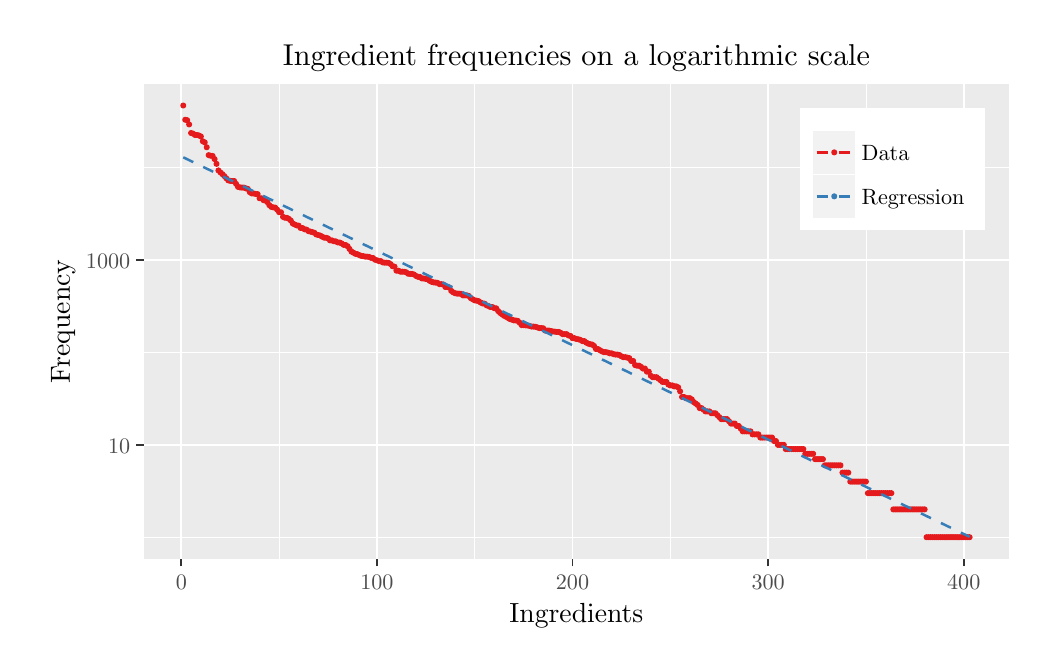
\begin{tikzpicture}[x=1pt,y=1pt]
\definecolor{fillColor}{RGB}{255,255,255}
\path[use as bounding box,fill=fillColor,fill opacity=0.00] (0,0) rectangle (360.07,222.54);
\begin{scope}
\path[clip] (  0.00,  0.00) rectangle (360.07,222.54);
\definecolor{drawColor}{RGB}{255,255,255}
\definecolor{fillColor}{RGB}{255,255,255}

\path[draw=drawColor,line width= 0.6pt,line join=round,line cap=round,fill=fillColor] (  0.00,  0.00) rectangle (360.07,222.54);
\end{scope}
\begin{scope}
\path[clip] ( 42.01, 30.62) rectangle (354.57,202.21);
\definecolor{fillColor}{gray}{0.92}

\path[fill=fillColor] ( 42.01, 30.62) rectangle (354.57,202.21);
\definecolor{drawColor}{RGB}{255,255,255}

\path[draw=drawColor,line width= 0.3pt,line join=round] ( 42.01, 38.42) --
	(354.57, 38.42);

\path[draw=drawColor,line width= 0.3pt,line join=round] ( 42.01,105.16) --
	(354.57,105.16);

\path[draw=drawColor,line width= 0.3pt,line join=round] ( 42.01,171.90) --
	(354.57,171.90);

\path[draw=drawColor,line width= 0.3pt,line join=round] ( 90.85, 30.62) --
	( 90.85,202.21);

\path[draw=drawColor,line width= 0.3pt,line join=round] (161.54, 30.62) --
	(161.54,202.21);

\path[draw=drawColor,line width= 0.3pt,line join=round] (232.22, 30.62) --
	(232.22,202.21);

\path[draw=drawColor,line width= 0.3pt,line join=round] (302.90, 30.62) --
	(302.90,202.21);

\path[draw=drawColor,line width= 0.6pt,line join=round] ( 42.01, 71.79) --
	(354.57, 71.79);

\path[draw=drawColor,line width= 0.6pt,line join=round] ( 42.01,138.53) --
	(354.57,138.53);

\path[draw=drawColor,line width= 0.6pt,line join=round] ( 55.51, 30.62) --
	( 55.51,202.21);

\path[draw=drawColor,line width= 0.6pt,line join=round] (126.20, 30.62) --
	(126.20,202.21);

\path[draw=drawColor,line width= 0.6pt,line join=round] (196.88, 30.62) --
	(196.88,202.21);

\path[draw=drawColor,line width= 0.6pt,line join=round] (267.56, 30.62) --
	(267.56,202.21);

\path[draw=drawColor,line width= 0.6pt,line join=round] (338.24, 30.62) --
	(338.24,202.21);
\definecolor{drawColor}{RGB}{228,26,28}
\definecolor{fillColor}{RGB}{228,26,28}

\path[draw=drawColor,line width= 0.4pt,line join=round,line cap=round,fill=fillColor] ( 56.22,194.41) circle (  0.89);

\path[draw=drawColor,line width= 0.4pt,line join=round,line cap=round,fill=fillColor] ( 56.93,189.27) circle (  0.89);

\path[draw=drawColor,line width= 0.4pt,line join=round,line cap=round,fill=fillColor] ( 57.63,189.11) circle (  0.89);

\path[draw=drawColor,line width= 0.4pt,line join=round,line cap=round,fill=fillColor] ( 58.34,187.57) circle (  0.89);

\path[draw=drawColor,line width= 0.4pt,line join=round,line cap=round,fill=fillColor] ( 59.05,184.48) circle (  0.89);

\path[draw=drawColor,line width= 0.4pt,line join=round,line cap=round,fill=fillColor] ( 59.75,184.25) circle (  0.89);

\path[draw=drawColor,line width= 0.4pt,line join=round,line cap=round,fill=fillColor] ( 60.46,183.76) circle (  0.89);

\path[draw=drawColor,line width= 0.4pt,line join=round,line cap=round,fill=fillColor] ( 61.17,183.75) circle (  0.89);

\path[draw=drawColor,line width= 0.4pt,line join=round,line cap=round,fill=fillColor] ( 61.87,183.59) circle (  0.89);

\path[draw=drawColor,line width= 0.4pt,line join=round,line cap=round,fill=fillColor] ( 62.58,183.23) circle (  0.89);

\path[draw=drawColor,line width= 0.4pt,line join=round,line cap=round,fill=fillColor] ( 63.29,181.49) circle (  0.89);

\path[draw=drawColor,line width= 0.4pt,line join=round,line cap=round,fill=fillColor] ( 63.99,181.08) circle (  0.89);

\path[draw=drawColor,line width= 0.4pt,line join=round,line cap=round,fill=fillColor] ( 64.70,179.32) circle (  0.89);

\path[draw=drawColor,line width= 0.4pt,line join=round,line cap=round,fill=fillColor] ( 65.41,176.48) circle (  0.89);

\path[draw=drawColor,line width= 0.4pt,line join=round,line cap=round,fill=fillColor] ( 66.11,176.26) circle (  0.89);

\path[draw=drawColor,line width= 0.4pt,line join=round,line cap=round,fill=fillColor] ( 66.82,176.18) circle (  0.89);

\path[draw=drawColor,line width= 0.4pt,line join=round,line cap=round,fill=fillColor] ( 67.53,175.05) circle (  0.89);

\path[draw=drawColor,line width= 0.4pt,line join=round,line cap=round,fill=fillColor] ( 68.24,173.33) circle (  0.89);

\path[draw=drawColor,line width= 0.4pt,line join=round,line cap=round,fill=fillColor] ( 68.94,170.95) circle (  0.89);

\path[draw=drawColor,line width= 0.4pt,line join=round,line cap=round,fill=fillColor] ( 69.65,170.22) circle (  0.89);

\path[draw=drawColor,line width= 0.4pt,line join=round,line cap=round,fill=fillColor] ( 70.36,169.62) circle (  0.89);

\path[draw=drawColor,line width= 0.4pt,line join=round,line cap=round,fill=fillColor] ( 71.06,168.91) circle (  0.89);

\path[draw=drawColor,line width= 0.4pt,line join=round,line cap=round,fill=fillColor] ( 71.77,168.10) circle (  0.89);

\path[draw=drawColor,line width= 0.4pt,line join=round,line cap=round,fill=fillColor] ( 72.48,167.37) circle (  0.89);

\path[draw=drawColor,line width= 0.4pt,line join=round,line cap=round,fill=fillColor] ( 73.18,167.18) circle (  0.89);

\path[draw=drawColor,line width= 0.4pt,line join=round,line cap=round,fill=fillColor] ( 73.89,167.14) circle (  0.89);

\path[draw=drawColor,line width= 0.4pt,line join=round,line cap=round,fill=fillColor] ( 74.60,167.14) circle (  0.89);

\path[draw=drawColor,line width= 0.4pt,line join=round,line cap=round,fill=fillColor] ( 75.30,166.10) circle (  0.89);

\path[draw=drawColor,line width= 0.4pt,line join=round,line cap=round,fill=fillColor] ( 76.01,165.00) circle (  0.89);

\path[draw=drawColor,line width= 0.4pt,line join=round,line cap=round,fill=fillColor] ( 76.72,164.82) circle (  0.89);

\path[draw=drawColor,line width= 0.4pt,line join=round,line cap=round,fill=fillColor] ( 77.42,164.76) circle (  0.89);

\path[draw=drawColor,line width= 0.4pt,line join=round,line cap=round,fill=fillColor] ( 78.13,164.75) circle (  0.89);

\path[draw=drawColor,line width= 0.4pt,line join=round,line cap=round,fill=fillColor] ( 78.84,164.47) circle (  0.89);

\path[draw=drawColor,line width= 0.4pt,line join=round,line cap=round,fill=fillColor] ( 79.54,164.28) circle (  0.89);

\path[draw=drawColor,line width= 0.4pt,line join=round,line cap=round,fill=fillColor] ( 80.25,163.11) circle (  0.89);

\path[draw=drawColor,line width= 0.4pt,line join=round,line cap=round,fill=fillColor] ( 80.96,162.65) circle (  0.89);

\path[draw=drawColor,line width= 0.4pt,line join=round,line cap=round,fill=fillColor] ( 81.67,162.64) circle (  0.89);

\path[draw=drawColor,line width= 0.4pt,line join=round,line cap=round,fill=fillColor] ( 82.37,162.45) circle (  0.89);

\path[draw=drawColor,line width= 0.4pt,line join=round,line cap=round,fill=fillColor] ( 83.08,162.40) circle (  0.89);

\path[draw=drawColor,line width= 0.4pt,line join=round,line cap=round,fill=fillColor] ( 83.79,160.90) circle (  0.89);

\path[draw=drawColor,line width= 0.4pt,line join=round,line cap=round,fill=fillColor] ( 84.49,160.89) circle (  0.89);

\path[draw=drawColor,line width= 0.4pt,line join=round,line cap=round,fill=fillColor] ( 85.20,160.22) circle (  0.89);

\path[draw=drawColor,line width= 0.4pt,line join=round,line cap=round,fill=fillColor] ( 85.91,160.05) circle (  0.89);

\path[draw=drawColor,line width= 0.4pt,line join=round,line cap=round,fill=fillColor] ( 86.61,159.50) circle (  0.89);

\path[draw=drawColor,line width= 0.4pt,line join=round,line cap=round,fill=fillColor] ( 87.32,158.40) circle (  0.89);

\path[draw=drawColor,line width= 0.4pt,line join=round,line cap=round,fill=fillColor] ( 88.03,157.78) circle (  0.89);

\path[draw=drawColor,line width= 0.4pt,line join=round,line cap=round,fill=fillColor] ( 88.73,157.61) circle (  0.89);

\path[draw=drawColor,line width= 0.4pt,line join=round,line cap=round,fill=fillColor] ( 89.44,157.51) circle (  0.89);

\path[draw=drawColor,line width= 0.4pt,line join=round,line cap=round,fill=fillColor] ( 90.15,156.78) circle (  0.89);

\path[draw=drawColor,line width= 0.4pt,line join=round,line cap=round,fill=fillColor] ( 90.85,155.86) circle (  0.89);

\path[draw=drawColor,line width= 0.4pt,line join=round,line cap=round,fill=fillColor] ( 91.56,155.82) circle (  0.89);

\path[draw=drawColor,line width= 0.4pt,line join=round,line cap=round,fill=fillColor] ( 92.27,154.18) circle (  0.89);

\path[draw=drawColor,line width= 0.4pt,line join=round,line cap=round,fill=fillColor] ( 92.97,153.85) circle (  0.89);

\path[draw=drawColor,line width= 0.4pt,line join=round,line cap=round,fill=fillColor] ( 93.68,153.82) circle (  0.89);

\path[draw=drawColor,line width= 0.4pt,line join=round,line cap=round,fill=fillColor] ( 94.39,153.45) circle (  0.89);

\path[draw=drawColor,line width= 0.4pt,line join=round,line cap=round,fill=fillColor] ( 95.09,152.82) circle (  0.89);

\path[draw=drawColor,line width= 0.4pt,line join=round,line cap=round,fill=fillColor] ( 95.80,151.76) circle (  0.89);

\path[draw=drawColor,line width= 0.4pt,line join=round,line cap=round,fill=fillColor] ( 96.51,151.42) circle (  0.89);

\path[draw=drawColor,line width= 0.4pt,line join=round,line cap=round,fill=fillColor] ( 97.22,151.08) circle (  0.89);

\path[draw=drawColor,line width= 0.4pt,line join=round,line cap=round,fill=fillColor] ( 97.92,151.00) circle (  0.89);

\path[draw=drawColor,line width= 0.4pt,line join=round,line cap=round,fill=fillColor] ( 98.63,150.15) circle (  0.89);

\path[draw=drawColor,line width= 0.4pt,line join=round,line cap=round,fill=fillColor] ( 99.34,150.13) circle (  0.89);

\path[draw=drawColor,line width= 0.4pt,line join=round,line cap=round,fill=fillColor] (100.04,149.68) circle (  0.89);

\path[draw=drawColor,line width= 0.4pt,line join=round,line cap=round,fill=fillColor] (100.75,149.56) circle (  0.89);

\path[draw=drawColor,line width= 0.4pt,line join=round,line cap=round,fill=fillColor] (101.46,149.03) circle (  0.89);

\path[draw=drawColor,line width= 0.4pt,line join=round,line cap=round,fill=fillColor] (102.16,148.85) circle (  0.89);

\path[draw=drawColor,line width= 0.4pt,line join=round,line cap=round,fill=fillColor] (102.87,148.68) circle (  0.89);

\path[draw=drawColor,line width= 0.4pt,line join=round,line cap=round,fill=fillColor] (103.58,148.43) circle (  0.89);

\path[draw=drawColor,line width= 0.4pt,line join=round,line cap=round,fill=fillColor] (104.28,147.80) circle (  0.89);

\path[draw=drawColor,line width= 0.4pt,line join=round,line cap=round,fill=fillColor] (104.99,147.62) circle (  0.89);

\path[draw=drawColor,line width= 0.4pt,line join=round,line cap=round,fill=fillColor] (105.70,147.43) circle (  0.89);

\path[draw=drawColor,line width= 0.4pt,line join=round,line cap=round,fill=fillColor] (106.40,147.01) circle (  0.89);

\path[draw=drawColor,line width= 0.4pt,line join=round,line cap=round,fill=fillColor] (107.11,146.67) circle (  0.89);

\path[draw=drawColor,line width= 0.4pt,line join=round,line cap=round,fill=fillColor] (107.82,146.62) circle (  0.89);

\path[draw=drawColor,line width= 0.4pt,line join=round,line cap=round,fill=fillColor] (108.52,146.39) circle (  0.89);

\path[draw=drawColor,line width= 0.4pt,line join=round,line cap=round,fill=fillColor] (109.23,145.70) circle (  0.89);

\path[draw=drawColor,line width= 0.4pt,line join=round,line cap=round,fill=fillColor] (109.94,145.67) circle (  0.89);

\path[draw=drawColor,line width= 0.4pt,line join=round,line cap=round,fill=fillColor] (110.64,145.37) circle (  0.89);

\path[draw=drawColor,line width= 0.4pt,line join=round,line cap=round,fill=fillColor] (111.35,145.30) circle (  0.89);

\path[draw=drawColor,line width= 0.4pt,line join=round,line cap=round,fill=fillColor] (112.06,144.94) circle (  0.89);

\path[draw=drawColor,line width= 0.4pt,line join=round,line cap=round,fill=fillColor] (112.77,144.89) circle (  0.89);

\path[draw=drawColor,line width= 0.4pt,line join=round,line cap=round,fill=fillColor] (113.47,144.57) circle (  0.89);

\path[draw=drawColor,line width= 0.4pt,line join=round,line cap=round,fill=fillColor] (114.18,144.07) circle (  0.89);

\path[draw=drawColor,line width= 0.4pt,line join=round,line cap=round,fill=fillColor] (114.89,144.00) circle (  0.89);

\path[draw=drawColor,line width= 0.4pt,line join=round,line cap=round,fill=fillColor] (115.59,143.57) circle (  0.89);

\path[draw=drawColor,line width= 0.4pt,line join=round,line cap=round,fill=fillColor] (116.30,142.57) circle (  0.89);

\path[draw=drawColor,line width= 0.4pt,line join=round,line cap=round,fill=fillColor] (117.01,141.60) circle (  0.89);

\path[draw=drawColor,line width= 0.4pt,line join=round,line cap=round,fill=fillColor] (117.71,141.23) circle (  0.89);

\path[draw=drawColor,line width= 0.4pt,line join=round,line cap=round,fill=fillColor] (118.42,140.82) circle (  0.89);

\path[draw=drawColor,line width= 0.4pt,line join=round,line cap=round,fill=fillColor] (119.13,140.69) circle (  0.89);

\path[draw=drawColor,line width= 0.4pt,line join=round,line cap=round,fill=fillColor] (119.83,140.38) circle (  0.89);

\path[draw=drawColor,line width= 0.4pt,line join=round,line cap=round,fill=fillColor] (120.54,140.08) circle (  0.89);

\path[draw=drawColor,line width= 0.4pt,line join=round,line cap=round,fill=fillColor] (121.25,139.98) circle (  0.89);

\path[draw=drawColor,line width= 0.4pt,line join=round,line cap=round,fill=fillColor] (121.95,139.82) circle (  0.89);

\path[draw=drawColor,line width= 0.4pt,line join=round,line cap=round,fill=fillColor] (122.66,139.79) circle (  0.89);

\path[draw=drawColor,line width= 0.4pt,line join=round,line cap=round,fill=fillColor] (123.37,139.70) circle (  0.89);

\path[draw=drawColor,line width= 0.4pt,line join=round,line cap=round,fill=fillColor] (124.07,139.37) circle (  0.89);

\path[draw=drawColor,line width= 0.4pt,line join=round,line cap=round,fill=fillColor] (124.78,139.32) circle (  0.89);

\path[draw=drawColor,line width= 0.4pt,line join=round,line cap=round,fill=fillColor] (125.49,138.70) circle (  0.89);

\path[draw=drawColor,line width= 0.4pt,line join=round,line cap=round,fill=fillColor] (126.20,138.50) circle (  0.89);

\path[draw=drawColor,line width= 0.4pt,line join=round,line cap=round,fill=fillColor] (126.90,138.19) circle (  0.89);

\path[draw=drawColor,line width= 0.4pt,line join=round,line cap=round,fill=fillColor] (127.61,138.18) circle (  0.89);

\path[draw=drawColor,line width= 0.4pt,line join=round,line cap=round,fill=fillColor] (128.32,137.71) circle (  0.89);

\path[draw=drawColor,line width= 0.4pt,line join=round,line cap=round,fill=fillColor] (129.02,137.63) circle (  0.89);

\path[draw=drawColor,line width= 0.4pt,line join=round,line cap=round,fill=fillColor] (129.73,137.63) circle (  0.89);

\path[draw=drawColor,line width= 0.4pt,line join=round,line cap=round,fill=fillColor] (130.44,137.55) circle (  0.89);

\path[draw=drawColor,line width= 0.4pt,line join=round,line cap=round,fill=fillColor] (131.14,137.11) circle (  0.89);

\path[draw=drawColor,line width= 0.4pt,line join=round,line cap=round,fill=fillColor] (131.85,136.33) circle (  0.89);

\path[draw=drawColor,line width= 0.4pt,line join=round,line cap=round,fill=fillColor] (132.56,136.17) circle (  0.89);

\path[draw=drawColor,line width= 0.4pt,line join=round,line cap=round,fill=fillColor] (133.26,134.72) circle (  0.89);

\path[draw=drawColor,line width= 0.4pt,line join=round,line cap=round,fill=fillColor] (133.97,134.72) circle (  0.89);

\path[draw=drawColor,line width= 0.4pt,line join=round,line cap=round,fill=fillColor] (134.68,134.36) circle (  0.89);

\path[draw=drawColor,line width= 0.4pt,line join=round,line cap=round,fill=fillColor] (135.38,134.36) circle (  0.89);

\path[draw=drawColor,line width= 0.4pt,line join=round,line cap=round,fill=fillColor] (136.09,134.34) circle (  0.89);

\path[draw=drawColor,line width= 0.4pt,line join=round,line cap=round,fill=fillColor] (136.80,134.15) circle (  0.89);

\path[draw=drawColor,line width= 0.4pt,line join=round,line cap=round,fill=fillColor] (137.50,133.61) circle (  0.89);

\path[draw=drawColor,line width= 0.4pt,line join=round,line cap=round,fill=fillColor] (138.21,133.57) circle (  0.89);

\path[draw=drawColor,line width= 0.4pt,line join=round,line cap=round,fill=fillColor] (138.92,133.55) circle (  0.89);

\path[draw=drawColor,line width= 0.4pt,line join=round,line cap=round,fill=fillColor] (139.62,133.34) circle (  0.89);

\path[draw=drawColor,line width= 0.4pt,line join=round,line cap=round,fill=fillColor] (140.33,132.83) circle (  0.89);

\path[draw=drawColor,line width= 0.4pt,line join=round,line cap=round,fill=fillColor] (141.04,132.51) circle (  0.89);

\path[draw=drawColor,line width= 0.4pt,line join=round,line cap=round,fill=fillColor] (141.75,132.46) circle (  0.89);

\path[draw=drawColor,line width= 0.4pt,line join=round,line cap=round,fill=fillColor] (142.45,131.92) circle (  0.89);

\path[draw=drawColor,line width= 0.4pt,line join=round,line cap=round,fill=fillColor] (143.16,131.92) circle (  0.89);

\path[draw=drawColor,line width= 0.4pt,line join=round,line cap=round,fill=fillColor] (143.87,131.74) circle (  0.89);

\path[draw=drawColor,line width= 0.4pt,line join=round,line cap=round,fill=fillColor] (144.57,131.60) circle (  0.89);

\path[draw=drawColor,line width= 0.4pt,line join=round,line cap=round,fill=fillColor] (145.28,131.05) circle (  0.89);

\path[draw=drawColor,line width= 0.4pt,line join=round,line cap=round,fill=fillColor] (145.99,130.68) circle (  0.89);

\path[draw=drawColor,line width= 0.4pt,line join=round,line cap=round,fill=fillColor] (146.69,130.51) circle (  0.89);

\path[draw=drawColor,line width= 0.4pt,line join=round,line cap=round,fill=fillColor] (147.40,130.43) circle (  0.89);

\path[draw=drawColor,line width= 0.4pt,line join=round,line cap=round,fill=fillColor] (148.11,130.31) circle (  0.89);

\path[draw=drawColor,line width= 0.4pt,line join=round,line cap=round,fill=fillColor] (148.81,129.87) circle (  0.89);

\path[draw=drawColor,line width= 0.4pt,line join=round,line cap=round,fill=fillColor] (149.52,129.84) circle (  0.89);

\path[draw=drawColor,line width= 0.4pt,line join=round,line cap=round,fill=fillColor] (150.23,129.71) circle (  0.89);

\path[draw=drawColor,line width= 0.4pt,line join=round,line cap=round,fill=fillColor] (150.93,128.83) circle (  0.89);

\path[draw=drawColor,line width= 0.4pt,line join=round,line cap=round,fill=fillColor] (151.64,128.80) circle (  0.89);

\path[draw=drawColor,line width= 0.4pt,line join=round,line cap=round,fill=fillColor] (152.35,128.66) circle (  0.89);

\path[draw=drawColor,line width= 0.4pt,line join=round,line cap=round,fill=fillColor] (153.05,127.43) circle (  0.89);

\path[draw=drawColor,line width= 0.4pt,line join=round,line cap=round,fill=fillColor] (153.76,126.92) circle (  0.89);

\path[draw=drawColor,line width= 0.4pt,line join=round,line cap=round,fill=fillColor] (154.47,126.57) circle (  0.89);

\path[draw=drawColor,line width= 0.4pt,line join=round,line cap=round,fill=fillColor] (155.18,126.43) circle (  0.89);

\path[draw=drawColor,line width= 0.4pt,line join=round,line cap=round,fill=fillColor] (155.88,126.43) circle (  0.89);

\path[draw=drawColor,line width= 0.4pt,line join=round,line cap=round,fill=fillColor] (156.59,126.37) circle (  0.89);

\path[draw=drawColor,line width= 0.4pt,line join=round,line cap=round,fill=fillColor] (157.30,125.82) circle (  0.89);

\path[draw=drawColor,line width= 0.4pt,line join=round,line cap=round,fill=fillColor] (158.00,125.82) circle (  0.89);

\path[draw=drawColor,line width= 0.4pt,line join=round,line cap=round,fill=fillColor] (158.71,125.82) circle (  0.89);

\path[draw=drawColor,line width= 0.4pt,line join=round,line cap=round,fill=fillColor] (159.42,125.57) circle (  0.89);

\path[draw=drawColor,line width= 0.4pt,line join=round,line cap=round,fill=fillColor] (160.12,124.81) circle (  0.89);

\path[draw=drawColor,line width= 0.4pt,line join=round,line cap=round,fill=fillColor] (160.83,124.39) circle (  0.89);

\path[draw=drawColor,line width= 0.4pt,line join=round,line cap=round,fill=fillColor] (161.54,124.00) circle (  0.89);

\path[draw=drawColor,line width= 0.4pt,line join=round,line cap=round,fill=fillColor] (162.24,123.88) circle (  0.89);

\path[draw=drawColor,line width= 0.4pt,line join=round,line cap=round,fill=fillColor] (162.95,123.72) circle (  0.89);

\path[draw=drawColor,line width= 0.4pt,line join=round,line cap=round,fill=fillColor] (163.66,123.23) circle (  0.89);

\path[draw=drawColor,line width= 0.4pt,line join=round,line cap=round,fill=fillColor] (164.36,122.90) circle (  0.89);

\path[draw=drawColor,line width= 0.4pt,line join=round,line cap=round,fill=fillColor] (165.07,122.81) circle (  0.89);

\path[draw=drawColor,line width= 0.4pt,line join=round,line cap=round,fill=fillColor] (165.78,122.24) circle (  0.89);

\path[draw=drawColor,line width= 0.4pt,line join=round,line cap=round,fill=fillColor] (166.48,121.97) circle (  0.89);

\path[draw=drawColor,line width= 0.4pt,line join=round,line cap=round,fill=fillColor] (167.19,121.60) circle (  0.89);

\path[draw=drawColor,line width= 0.4pt,line join=round,line cap=round,fill=fillColor] (167.90,121.60) circle (  0.89);

\path[draw=drawColor,line width= 0.4pt,line join=round,line cap=round,fill=fillColor] (168.60,121.18) circle (  0.89);

\path[draw=drawColor,line width= 0.4pt,line join=round,line cap=round,fill=fillColor] (169.31,121.13) circle (  0.89);

\path[draw=drawColor,line width= 0.4pt,line join=round,line cap=round,fill=fillColor] (170.02,120.13) circle (  0.89);

\path[draw=drawColor,line width= 0.4pt,line join=round,line cap=round,fill=fillColor] (170.73,119.45) circle (  0.89);

\path[draw=drawColor,line width= 0.4pt,line join=round,line cap=round,fill=fillColor] (171.43,118.95) circle (  0.89);

\path[draw=drawColor,line width= 0.4pt,line join=round,line cap=round,fill=fillColor] (172.14,118.44) circle (  0.89);

\path[draw=drawColor,line width= 0.4pt,line join=round,line cap=round,fill=fillColor] (172.85,118.09) circle (  0.89);

\path[draw=drawColor,line width= 0.4pt,line join=round,line cap=round,fill=fillColor] (173.55,117.67) circle (  0.89);

\path[draw=drawColor,line width= 0.4pt,line join=round,line cap=round,fill=fillColor] (174.26,117.23) circle (  0.89);

\path[draw=drawColor,line width= 0.4pt,line join=round,line cap=round,fill=fillColor] (174.97,117.04) circle (  0.89);

\path[draw=drawColor,line width= 0.4pt,line join=round,line cap=round,fill=fillColor] (175.67,116.78) circle (  0.89);

\path[draw=drawColor,line width= 0.4pt,line join=round,line cap=round,fill=fillColor] (176.38,116.72) circle (  0.89);

\path[draw=drawColor,line width= 0.4pt,line join=round,line cap=round,fill=fillColor] (177.09,116.59) circle (  0.89);

\path[draw=drawColor,line width= 0.4pt,line join=round,line cap=round,fill=fillColor] (177.79,115.91) circle (  0.89);

\path[draw=drawColor,line width= 0.4pt,line join=round,line cap=round,fill=fillColor] (178.50,115.06) circle (  0.89);

\path[draw=drawColor,line width= 0.4pt,line join=round,line cap=round,fill=fillColor] (179.21,115.06) circle (  0.89);

\path[draw=drawColor,line width= 0.4pt,line join=round,line cap=round,fill=fillColor] (179.91,114.99) circle (  0.89);

\path[draw=drawColor,line width= 0.4pt,line join=round,line cap=round,fill=fillColor] (180.62,114.91) circle (  0.89);

\path[draw=drawColor,line width= 0.4pt,line join=round,line cap=round,fill=fillColor] (181.33,114.76) circle (  0.89);

\path[draw=drawColor,line width= 0.4pt,line join=round,line cap=round,fill=fillColor] (182.03,114.54) circle (  0.89);

\path[draw=drawColor,line width= 0.4pt,line join=round,line cap=round,fill=fillColor] (182.74,114.54) circle (  0.89);

\path[draw=drawColor,line width= 0.4pt,line join=round,line cap=round,fill=fillColor] (183.45,114.46) circle (  0.89);

\path[draw=drawColor,line width= 0.4pt,line join=round,line cap=round,fill=fillColor] (184.15,114.23) circle (  0.89);

\path[draw=drawColor,line width= 0.4pt,line join=round,line cap=round,fill=fillColor] (184.86,114.00) circle (  0.89);

\path[draw=drawColor,line width= 0.4pt,line join=round,line cap=round,fill=fillColor] (185.57,114.00) circle (  0.89);

\path[draw=drawColor,line width= 0.4pt,line join=round,line cap=round,fill=fillColor] (186.28,113.92) circle (  0.89);

\path[draw=drawColor,line width= 0.4pt,line join=round,line cap=round,fill=fillColor] (186.98,113.10) circle (  0.89);

\path[draw=drawColor,line width= 0.4pt,line join=round,line cap=round,fill=fillColor] (187.69,113.10) circle (  0.89);

\path[draw=drawColor,line width= 0.4pt,line join=round,line cap=round,fill=fillColor] (188.40,113.10) circle (  0.89);

\path[draw=drawColor,line width= 0.4pt,line join=round,line cap=round,fill=fillColor] (189.10,112.94) circle (  0.89);

\path[draw=drawColor,line width= 0.4pt,line join=round,line cap=round,fill=fillColor] (189.81,112.76) circle (  0.89);

\path[draw=drawColor,line width= 0.4pt,line join=round,line cap=round,fill=fillColor] (190.52,112.68) circle (  0.89);

\path[draw=drawColor,line width= 0.4pt,line join=round,line cap=round,fill=fillColor] (191.22,112.59) circle (  0.89);

\path[draw=drawColor,line width= 0.4pt,line join=round,line cap=round,fill=fillColor] (191.93,112.59) circle (  0.89);

\path[draw=drawColor,line width= 0.4pt,line join=round,line cap=round,fill=fillColor] (192.64,112.24) circle (  0.89);

\path[draw=drawColor,line width= 0.4pt,line join=round,line cap=round,fill=fillColor] (193.34,111.79) circle (  0.89);

\path[draw=drawColor,line width= 0.4pt,line join=round,line cap=round,fill=fillColor] (194.05,111.79) circle (  0.89);

\path[draw=drawColor,line width= 0.4pt,line join=round,line cap=round,fill=fillColor] (194.76,111.79) circle (  0.89);

\path[draw=drawColor,line width= 0.4pt,line join=round,line cap=round,fill=fillColor] (195.46,111.32) circle (  0.89);

\path[draw=drawColor,line width= 0.4pt,line join=round,line cap=round,fill=fillColor] (196.17,111.13) circle (  0.89);

\path[draw=drawColor,line width= 0.4pt,line join=round,line cap=round,fill=fillColor] (196.88,110.34) circle (  0.89);

\path[draw=drawColor,line width= 0.4pt,line join=round,line cap=round,fill=fillColor] (197.58,110.34) circle (  0.89);

\path[draw=drawColor,line width= 0.4pt,line join=round,line cap=round,fill=fillColor] (198.29,110.04) circle (  0.89);

\path[draw=drawColor,line width= 0.4pt,line join=round,line cap=round,fill=fillColor] (199.00,109.93) circle (  0.89);

\path[draw=drawColor,line width= 0.4pt,line join=round,line cap=round,fill=fillColor] (199.71,109.72) circle (  0.89);

\path[draw=drawColor,line width= 0.4pt,line join=round,line cap=round,fill=fillColor] (200.41,109.29) circle (  0.89);

\path[draw=drawColor,line width= 0.4pt,line join=round,line cap=round,fill=fillColor] (201.12,109.29) circle (  0.89);

\path[draw=drawColor,line width= 0.4pt,line join=round,line cap=round,fill=fillColor] (201.83,108.74) circle (  0.89);

\path[draw=drawColor,line width= 0.4pt,line join=round,line cap=round,fill=fillColor] (202.53,108.39) circle (  0.89);

\path[draw=drawColor,line width= 0.4pt,line join=round,line cap=round,fill=fillColor] (203.24,108.16) circle (  0.89);

\path[draw=drawColor,line width= 0.4pt,line join=round,line cap=round,fill=fillColor] (203.95,108.04) circle (  0.89);

\path[draw=drawColor,line width= 0.4pt,line join=round,line cap=round,fill=fillColor] (204.65,107.56) circle (  0.89);

\path[draw=drawColor,line width= 0.4pt,line join=round,line cap=round,fill=fillColor] (205.36,106.41) circle (  0.89);

\path[draw=drawColor,line width= 0.4pt,line join=round,line cap=round,fill=fillColor] (206.07,106.41) circle (  0.89);

\path[draw=drawColor,line width= 0.4pt,line join=round,line cap=round,fill=fillColor] (206.77,106.00) circle (  0.89);

\path[draw=drawColor,line width= 0.4pt,line join=round,line cap=round,fill=fillColor] (207.48,105.59) circle (  0.89);

\path[draw=drawColor,line width= 0.4pt,line join=round,line cap=round,fill=fillColor] (208.19,105.30) circle (  0.89);

\path[draw=drawColor,line width= 0.4pt,line join=round,line cap=round,fill=fillColor] (208.89,105.30) circle (  0.89);

\path[draw=drawColor,line width= 0.4pt,line join=round,line cap=round,fill=fillColor] (209.60,105.16) circle (  0.89);

\path[draw=drawColor,line width= 0.4pt,line join=round,line cap=round,fill=fillColor] (210.31,104.87) circle (  0.89);

\path[draw=drawColor,line width= 0.4pt,line join=round,line cap=round,fill=fillColor] (211.01,104.87) circle (  0.89);

\path[draw=drawColor,line width= 0.4pt,line join=round,line cap=round,fill=fillColor] (211.72,104.57) circle (  0.89);

\path[draw=drawColor,line width= 0.4pt,line join=round,line cap=round,fill=fillColor] (212.43,104.42) circle (  0.89);

\path[draw=drawColor,line width= 0.4pt,line join=round,line cap=round,fill=fillColor] (213.13,104.42) circle (  0.89);

\path[draw=drawColor,line width= 0.4pt,line join=round,line cap=round,fill=fillColor] (213.84,104.26) circle (  0.89);

\path[draw=drawColor,line width= 0.4pt,line join=round,line cap=round,fill=fillColor] (214.55,103.79) circle (  0.89);

\path[draw=drawColor,line width= 0.4pt,line join=round,line cap=round,fill=fillColor] (215.26,103.47) circle (  0.89);

\path[draw=drawColor,line width= 0.4pt,line join=round,line cap=round,fill=fillColor] (215.96,103.47) circle (  0.89);

\path[draw=drawColor,line width= 0.4pt,line join=round,line cap=round,fill=fillColor] (216.67,103.31) circle (  0.89);

\path[draw=drawColor,line width= 0.4pt,line join=round,line cap=round,fill=fillColor] (217.38,103.14) circle (  0.89);

\path[draw=drawColor,line width= 0.4pt,line join=round,line cap=round,fill=fillColor] (218.08,102.11) circle (  0.89);

\path[draw=drawColor,line width= 0.4pt,line join=round,line cap=round,fill=fillColor] (218.79,102.11) circle (  0.89);

\path[draw=drawColor,line width= 0.4pt,line join=round,line cap=round,fill=fillColor] (219.50,100.60) circle (  0.89);

\path[draw=drawColor,line width= 0.4pt,line join=round,line cap=round,fill=fillColor] (220.20,100.40) circle (  0.89);

\path[draw=drawColor,line width= 0.4pt,line join=round,line cap=round,fill=fillColor] (220.91,100.40) circle (  0.89);

\path[draw=drawColor,line width= 0.4pt,line join=round,line cap=round,fill=fillColor] (221.62, 99.99) circle (  0.89);

\path[draw=drawColor,line width= 0.4pt,line join=round,line cap=round,fill=fillColor] (222.32, 99.36) circle (  0.89);

\path[draw=drawColor,line width= 0.4pt,line join=round,line cap=round,fill=fillColor] (223.03, 99.36) circle (  0.89);

\path[draw=drawColor,line width= 0.4pt,line join=round,line cap=round,fill=fillColor] (223.74, 98.23) circle (  0.89);

\path[draw=drawColor,line width= 0.4pt,line join=round,line cap=round,fill=fillColor] (224.44, 98.23) circle (  0.89);

\path[draw=drawColor,line width= 0.4pt,line join=round,line cap=round,fill=fillColor] (225.15, 96.76) circle (  0.89);

\path[draw=drawColor,line width= 0.4pt,line join=round,line cap=round,fill=fillColor] (225.86, 96.23) circle (  0.89);

\path[draw=drawColor,line width= 0.4pt,line join=round,line cap=round,fill=fillColor] (226.56, 96.23) circle (  0.89);

\path[draw=drawColor,line width= 0.4pt,line join=round,line cap=round,fill=fillColor] (227.27, 96.23) circle (  0.89);

\path[draw=drawColor,line width= 0.4pt,line join=round,line cap=round,fill=fillColor] (227.98, 95.68) circle (  0.89);

\path[draw=drawColor,line width= 0.4pt,line join=round,line cap=round,fill=fillColor] (228.69, 95.12) circle (  0.89);

\path[draw=drawColor,line width= 0.4pt,line join=round,line cap=round,fill=fillColor] (229.39, 94.52) circle (  0.89);

\path[draw=drawColor,line width= 0.4pt,line join=round,line cap=round,fill=fillColor] (230.10, 94.52) circle (  0.89);

\path[draw=drawColor,line width= 0.4pt,line join=round,line cap=round,fill=fillColor] (230.81, 94.52) circle (  0.89);

\path[draw=drawColor,line width= 0.4pt,line join=round,line cap=round,fill=fillColor] (231.51, 93.59) circle (  0.89);

\path[draw=drawColor,line width= 0.4pt,line join=round,line cap=round,fill=fillColor] (232.22, 93.26) circle (  0.89);

\path[draw=drawColor,line width= 0.4pt,line join=round,line cap=round,fill=fillColor] (232.93, 93.26) circle (  0.89);

\path[draw=drawColor,line width= 0.4pt,line join=round,line cap=round,fill=fillColor] (233.63, 92.93) circle (  0.89);

\path[draw=drawColor,line width= 0.4pt,line join=round,line cap=round,fill=fillColor] (234.34, 92.93) circle (  0.89);

\path[draw=drawColor,line width= 0.4pt,line join=round,line cap=round,fill=fillColor] (235.05, 92.59) circle (  0.89);

\path[draw=drawColor,line width= 0.4pt,line join=round,line cap=round,fill=fillColor] (235.75, 91.14) circle (  0.89);

\path[draw=drawColor,line width= 0.4pt,line join=round,line cap=round,fill=fillColor] (236.46, 89.09) circle (  0.89);

\path[draw=drawColor,line width= 0.4pt,line join=round,line cap=round,fill=fillColor] (237.17, 89.09) circle (  0.89);

\path[draw=drawColor,line width= 0.4pt,line join=round,line cap=round,fill=fillColor] (237.87, 88.65) circle (  0.89);

\path[draw=drawColor,line width= 0.4pt,line join=round,line cap=round,fill=fillColor] (238.58, 88.65) circle (  0.89);

\path[draw=drawColor,line width= 0.4pt,line join=round,line cap=round,fill=fillColor] (239.29, 88.65) circle (  0.89);

\path[draw=drawColor,line width= 0.4pt,line join=round,line cap=round,fill=fillColor] (239.99, 88.19) circle (  0.89);

\path[draw=drawColor,line width= 0.4pt,line join=round,line cap=round,fill=fillColor] (240.70, 87.22) circle (  0.89);

\path[draw=drawColor,line width= 0.4pt,line join=round,line cap=round,fill=fillColor] (241.41, 86.71) circle (  0.89);

\path[draw=drawColor,line width= 0.4pt,line join=round,line cap=round,fill=fillColor] (242.11, 86.19) circle (  0.89);

\path[draw=drawColor,line width= 0.4pt,line join=round,line cap=round,fill=fillColor] (242.82, 85.07) circle (  0.89);

\path[draw=drawColor,line width= 0.4pt,line join=round,line cap=round,fill=fillColor] (243.53, 85.07) circle (  0.89);

\path[draw=drawColor,line width= 0.4pt,line join=round,line cap=round,fill=fillColor] (244.24, 84.48) circle (  0.89);

\path[draw=drawColor,line width= 0.4pt,line join=round,line cap=round,fill=fillColor] (244.94, 83.86) circle (  0.89);

\path[draw=drawColor,line width= 0.4pt,line join=round,line cap=round,fill=fillColor] (245.65, 83.86) circle (  0.89);

\path[draw=drawColor,line width= 0.4pt,line join=round,line cap=round,fill=fillColor] (246.36, 83.86) circle (  0.89);

\path[draw=drawColor,line width= 0.4pt,line join=round,line cap=round,fill=fillColor] (247.06, 83.22) circle (  0.89);

\path[draw=drawColor,line width= 0.4pt,line join=round,line cap=round,fill=fillColor] (247.77, 83.22) circle (  0.89);

\path[draw=drawColor,line width= 0.4pt,line join=round,line cap=round,fill=fillColor] (248.48, 83.22) circle (  0.89);

\path[draw=drawColor,line width= 0.4pt,line join=round,line cap=round,fill=fillColor] (249.18, 82.54) circle (  0.89);

\path[draw=drawColor,line width= 0.4pt,line join=round,line cap=round,fill=fillColor] (249.89, 81.84) circle (  0.89);

\path[draw=drawColor,line width= 0.4pt,line join=round,line cap=round,fill=fillColor] (250.60, 81.09) circle (  0.89);

\path[draw=drawColor,line width= 0.4pt,line join=round,line cap=round,fill=fillColor] (251.30, 81.09) circle (  0.89);

\path[draw=drawColor,line width= 0.4pt,line join=round,line cap=round,fill=fillColor] (252.01, 81.09) circle (  0.89);

\path[draw=drawColor,line width= 0.4pt,line join=round,line cap=round,fill=fillColor] (252.72, 81.09) circle (  0.89);

\path[draw=drawColor,line width= 0.4pt,line join=round,line cap=round,fill=fillColor] (253.42, 80.31) circle (  0.89);

\path[draw=drawColor,line width= 0.4pt,line join=round,line cap=round,fill=fillColor] (254.13, 79.48) circle (  0.89);

\path[draw=drawColor,line width= 0.4pt,line join=round,line cap=round,fill=fillColor] (254.84, 79.48) circle (  0.89);

\path[draw=drawColor,line width= 0.4pt,line join=round,line cap=round,fill=fillColor] (255.54, 79.48) circle (  0.89);

\path[draw=drawColor,line width= 0.4pt,line join=round,line cap=round,fill=fillColor] (256.25, 78.60) circle (  0.89);

\path[draw=drawColor,line width= 0.4pt,line join=round,line cap=round,fill=fillColor] (256.96, 78.60) circle (  0.89);

\path[draw=drawColor,line width= 0.4pt,line join=round,line cap=round,fill=fillColor] (257.66, 77.67) circle (  0.89);

\path[draw=drawColor,line width= 0.4pt,line join=round,line cap=round,fill=fillColor] (258.37, 76.67) circle (  0.89);

\path[draw=drawColor,line width= 0.4pt,line join=round,line cap=round,fill=fillColor] (259.08, 76.67) circle (  0.89);

\path[draw=drawColor,line width= 0.4pt,line join=round,line cap=round,fill=fillColor] (259.79, 76.67) circle (  0.89);

\path[draw=drawColor,line width= 0.4pt,line join=round,line cap=round,fill=fillColor] (260.49, 76.67) circle (  0.89);

\path[draw=drawColor,line width= 0.4pt,line join=round,line cap=round,fill=fillColor] (261.20, 76.67) circle (  0.89);

\path[draw=drawColor,line width= 0.4pt,line join=round,line cap=round,fill=fillColor] (261.91, 75.59) circle (  0.89);

\path[draw=drawColor,line width= 0.4pt,line join=round,line cap=round,fill=fillColor] (262.61, 75.59) circle (  0.89);

\path[draw=drawColor,line width= 0.4pt,line join=round,line cap=round,fill=fillColor] (263.32, 75.59) circle (  0.89);

\path[draw=drawColor,line width= 0.4pt,line join=round,line cap=round,fill=fillColor] (264.03, 75.59) circle (  0.89);

\path[draw=drawColor,line width= 0.4pt,line join=round,line cap=round,fill=fillColor] (264.73, 74.43) circle (  0.89);

\path[draw=drawColor,line width= 0.4pt,line join=round,line cap=round,fill=fillColor] (265.44, 74.43) circle (  0.89);

\path[draw=drawColor,line width= 0.4pt,line join=round,line cap=round,fill=fillColor] (266.15, 74.43) circle (  0.89);

\path[draw=drawColor,line width= 0.4pt,line join=round,line cap=round,fill=fillColor] (266.85, 74.43) circle (  0.89);

\path[draw=drawColor,line width= 0.4pt,line join=round,line cap=round,fill=fillColor] (267.56, 74.43) circle (  0.89);

\path[draw=drawColor,line width= 0.4pt,line join=round,line cap=round,fill=fillColor] (268.27, 74.43) circle (  0.89);

\path[draw=drawColor,line width= 0.4pt,line join=round,line cap=round,fill=fillColor] (268.97, 74.43) circle (  0.89);

\path[draw=drawColor,line width= 0.4pt,line join=round,line cap=round,fill=fillColor] (269.68, 73.17) circle (  0.89);

\path[draw=drawColor,line width= 0.4pt,line join=round,line cap=round,fill=fillColor] (270.39, 73.17) circle (  0.89);

\path[draw=drawColor,line width= 0.4pt,line join=round,line cap=round,fill=fillColor] (271.09, 71.79) circle (  0.89);

\path[draw=drawColor,line width= 0.4pt,line join=round,line cap=round,fill=fillColor] (271.80, 71.79) circle (  0.89);

\path[draw=drawColor,line width= 0.4pt,line join=round,line cap=round,fill=fillColor] (272.51, 71.79) circle (  0.89);

\path[draw=drawColor,line width= 0.4pt,line join=round,line cap=round,fill=fillColor] (273.22, 71.79) circle (  0.89);

\path[draw=drawColor,line width= 0.4pt,line join=round,line cap=round,fill=fillColor] (273.92, 70.27) circle (  0.89);

\path[draw=drawColor,line width= 0.4pt,line join=round,line cap=round,fill=fillColor] (274.63, 70.27) circle (  0.89);

\path[draw=drawColor,line width= 0.4pt,line join=round,line cap=round,fill=fillColor] (275.34, 70.27) circle (  0.89);

\path[draw=drawColor,line width= 0.4pt,line join=round,line cap=round,fill=fillColor] (276.04, 70.27) circle (  0.89);

\path[draw=drawColor,line width= 0.4pt,line join=round,line cap=round,fill=fillColor] (276.75, 70.27) circle (  0.89);

\path[draw=drawColor,line width= 0.4pt,line join=round,line cap=round,fill=fillColor] (277.46, 70.27) circle (  0.89);

\path[draw=drawColor,line width= 0.4pt,line join=round,line cap=round,fill=fillColor] (278.16, 70.27) circle (  0.89);

\path[draw=drawColor,line width= 0.4pt,line join=round,line cap=round,fill=fillColor] (278.87, 70.27) circle (  0.89);

\path[draw=drawColor,line width= 0.4pt,line join=round,line cap=round,fill=fillColor] (279.58, 70.27) circle (  0.89);

\path[draw=drawColor,line width= 0.4pt,line join=round,line cap=round,fill=fillColor] (280.28, 70.27) circle (  0.89);

\path[draw=drawColor,line width= 0.4pt,line join=round,line cap=round,fill=fillColor] (280.99, 68.56) circle (  0.89);

\path[draw=drawColor,line width= 0.4pt,line join=round,line cap=round,fill=fillColor] (281.70, 68.56) circle (  0.89);

\path[draw=drawColor,line width= 0.4pt,line join=round,line cap=round,fill=fillColor] (282.40, 68.56) circle (  0.89);

\path[draw=drawColor,line width= 0.4pt,line join=round,line cap=round,fill=fillColor] (283.11, 68.56) circle (  0.89);

\path[draw=drawColor,line width= 0.4pt,line join=round,line cap=round,fill=fillColor] (283.82, 68.56) circle (  0.89);

\path[draw=drawColor,line width= 0.4pt,line join=round,line cap=round,fill=fillColor] (284.52, 66.62) circle (  0.89);

\path[draw=drawColor,line width= 0.4pt,line join=round,line cap=round,fill=fillColor] (285.23, 66.62) circle (  0.89);

\path[draw=drawColor,line width= 0.4pt,line join=round,line cap=round,fill=fillColor] (285.94, 66.62) circle (  0.89);

\path[draw=drawColor,line width= 0.4pt,line join=round,line cap=round,fill=fillColor] (286.64, 66.62) circle (  0.89);

\path[draw=drawColor,line width= 0.4pt,line join=round,line cap=round,fill=fillColor] (287.35, 66.62) circle (  0.89);

\path[draw=drawColor,line width= 0.4pt,line join=round,line cap=round,fill=fillColor] (288.06, 64.39) circle (  0.89);

\path[draw=drawColor,line width= 0.4pt,line join=round,line cap=round,fill=fillColor] (288.77, 64.39) circle (  0.89);

\path[draw=drawColor,line width= 0.4pt,line join=round,line cap=round,fill=fillColor] (289.47, 64.39) circle (  0.89);

\path[draw=drawColor,line width= 0.4pt,line join=round,line cap=round,fill=fillColor] (290.18, 64.39) circle (  0.89);

\path[draw=drawColor,line width= 0.4pt,line join=round,line cap=round,fill=fillColor] (290.89, 64.39) circle (  0.89);

\path[draw=drawColor,line width= 0.4pt,line join=round,line cap=round,fill=fillColor] (291.59, 64.39) circle (  0.89);

\path[draw=drawColor,line width= 0.4pt,line join=round,line cap=round,fill=fillColor] (292.30, 64.39) circle (  0.89);

\path[draw=drawColor,line width= 0.4pt,line join=round,line cap=round,fill=fillColor] (293.01, 64.39) circle (  0.89);

\path[draw=drawColor,line width= 0.4pt,line join=round,line cap=round,fill=fillColor] (293.71, 64.39) circle (  0.89);

\path[draw=drawColor,line width= 0.4pt,line join=round,line cap=round,fill=fillColor] (294.42, 61.75) circle (  0.89);

\path[draw=drawColor,line width= 0.4pt,line join=round,line cap=round,fill=fillColor] (295.13, 61.75) circle (  0.89);

\path[draw=drawColor,line width= 0.4pt,line join=round,line cap=round,fill=fillColor] (295.83, 61.75) circle (  0.89);

\path[draw=drawColor,line width= 0.4pt,line join=round,line cap=round,fill=fillColor] (296.54, 61.75) circle (  0.89);

\path[draw=drawColor,line width= 0.4pt,line join=round,line cap=round,fill=fillColor] (297.25, 58.51) circle (  0.89);

\path[draw=drawColor,line width= 0.4pt,line join=round,line cap=round,fill=fillColor] (297.95, 58.51) circle (  0.89);

\path[draw=drawColor,line width= 0.4pt,line join=round,line cap=round,fill=fillColor] (298.66, 58.51) circle (  0.89);

\path[draw=drawColor,line width= 0.4pt,line join=round,line cap=round,fill=fillColor] (299.37, 58.51) circle (  0.89);

\path[draw=drawColor,line width= 0.4pt,line join=round,line cap=round,fill=fillColor] (300.07, 58.51) circle (  0.89);

\path[draw=drawColor,line width= 0.4pt,line join=round,line cap=round,fill=fillColor] (300.78, 58.51) circle (  0.89);

\path[draw=drawColor,line width= 0.4pt,line join=round,line cap=round,fill=fillColor] (301.49, 58.51) circle (  0.89);

\path[draw=drawColor,line width= 0.4pt,line join=round,line cap=round,fill=fillColor] (302.19, 58.51) circle (  0.89);

\path[draw=drawColor,line width= 0.4pt,line join=round,line cap=round,fill=fillColor] (302.90, 58.51) circle (  0.89);

\path[draw=drawColor,line width= 0.4pt,line join=round,line cap=round,fill=fillColor] (303.61, 54.34) circle (  0.89);

\path[draw=drawColor,line width= 0.4pt,line join=round,line cap=round,fill=fillColor] (304.32, 54.34) circle (  0.89);

\path[draw=drawColor,line width= 0.4pt,line join=round,line cap=round,fill=fillColor] (305.02, 54.34) circle (  0.89);

\path[draw=drawColor,line width= 0.4pt,line join=round,line cap=round,fill=fillColor] (305.73, 54.34) circle (  0.89);

\path[draw=drawColor,line width= 0.4pt,line join=round,line cap=round,fill=fillColor] (306.44, 54.34) circle (  0.89);

\path[draw=drawColor,line width= 0.4pt,line join=round,line cap=round,fill=fillColor] (307.14, 54.34) circle (  0.89);

\path[draw=drawColor,line width= 0.4pt,line join=round,line cap=round,fill=fillColor] (307.85, 54.34) circle (  0.89);

\path[draw=drawColor,line width= 0.4pt,line join=round,line cap=round,fill=fillColor] (308.56, 54.34) circle (  0.89);

\path[draw=drawColor,line width= 0.4pt,line join=round,line cap=round,fill=fillColor] (309.26, 54.34) circle (  0.89);

\path[draw=drawColor,line width= 0.4pt,line join=round,line cap=round,fill=fillColor] (309.97, 54.34) circle (  0.89);

\path[draw=drawColor,line width= 0.4pt,line join=round,line cap=round,fill=fillColor] (310.68, 54.34) circle (  0.89);

\path[draw=drawColor,line width= 0.4pt,line join=round,line cap=round,fill=fillColor] (311.38, 54.34) circle (  0.89);

\path[draw=drawColor,line width= 0.4pt,line join=round,line cap=round,fill=fillColor] (312.09, 54.34) circle (  0.89);

\path[draw=drawColor,line width= 0.4pt,line join=round,line cap=round,fill=fillColor] (312.80, 48.47) circle (  0.89);

\path[draw=drawColor,line width= 0.4pt,line join=round,line cap=round,fill=fillColor] (313.50, 48.47) circle (  0.89);

\path[draw=drawColor,line width= 0.4pt,line join=round,line cap=round,fill=fillColor] (314.21, 48.47) circle (  0.89);

\path[draw=drawColor,line width= 0.4pt,line join=round,line cap=round,fill=fillColor] (314.92, 48.47) circle (  0.89);

\path[draw=drawColor,line width= 0.4pt,line join=round,line cap=round,fill=fillColor] (315.62, 48.47) circle (  0.89);

\path[draw=drawColor,line width= 0.4pt,line join=round,line cap=round,fill=fillColor] (316.33, 48.47) circle (  0.89);

\path[draw=drawColor,line width= 0.4pt,line join=round,line cap=round,fill=fillColor] (317.04, 48.47) circle (  0.89);

\path[draw=drawColor,line width= 0.4pt,line join=round,line cap=round,fill=fillColor] (317.75, 48.47) circle (  0.89);

\path[draw=drawColor,line width= 0.4pt,line join=round,line cap=round,fill=fillColor] (318.45, 48.47) circle (  0.89);

\path[draw=drawColor,line width= 0.4pt,line join=round,line cap=round,fill=fillColor] (319.16, 48.47) circle (  0.89);

\path[draw=drawColor,line width= 0.4pt,line join=round,line cap=round,fill=fillColor] (319.87, 48.47) circle (  0.89);

\path[draw=drawColor,line width= 0.4pt,line join=round,line cap=round,fill=fillColor] (320.57, 48.47) circle (  0.89);

\path[draw=drawColor,line width= 0.4pt,line join=round,line cap=round,fill=fillColor] (321.28, 48.47) circle (  0.89);

\path[draw=drawColor,line width= 0.4pt,line join=round,line cap=round,fill=fillColor] (321.99, 48.47) circle (  0.89);

\path[draw=drawColor,line width= 0.4pt,line join=round,line cap=round,fill=fillColor] (322.69, 48.47) circle (  0.89);

\path[draw=drawColor,line width= 0.4pt,line join=round,line cap=round,fill=fillColor] (323.40, 48.47) circle (  0.89);

\path[draw=drawColor,line width= 0.4pt,line join=round,line cap=round,fill=fillColor] (324.11, 48.47) circle (  0.89);

\path[draw=drawColor,line width= 0.4pt,line join=round,line cap=round,fill=fillColor] (324.81, 38.42) circle (  0.89);

\path[draw=drawColor,line width= 0.4pt,line join=round,line cap=round,fill=fillColor] (325.52, 38.42) circle (  0.89);

\path[draw=drawColor,line width= 0.4pt,line join=round,line cap=round,fill=fillColor] (326.23, 38.42) circle (  0.89);

\path[draw=drawColor,line width= 0.4pt,line join=round,line cap=round,fill=fillColor] (326.93, 38.42) circle (  0.89);

\path[draw=drawColor,line width= 0.4pt,line join=round,line cap=round,fill=fillColor] (327.64, 38.42) circle (  0.89);

\path[draw=drawColor,line width= 0.4pt,line join=round,line cap=round,fill=fillColor] (328.35, 38.42) circle (  0.89);

\path[draw=drawColor,line width= 0.4pt,line join=round,line cap=round,fill=fillColor] (329.05, 38.42) circle (  0.89);

\path[draw=drawColor,line width= 0.4pt,line join=round,line cap=round,fill=fillColor] (329.76, 38.42) circle (  0.89);

\path[draw=drawColor,line width= 0.4pt,line join=round,line cap=round,fill=fillColor] (330.47, 38.42) circle (  0.89);

\path[draw=drawColor,line width= 0.4pt,line join=round,line cap=round,fill=fillColor] (331.17, 38.42) circle (  0.89);

\path[draw=drawColor,line width= 0.4pt,line join=round,line cap=round,fill=fillColor] (331.88, 38.42) circle (  0.89);

\path[draw=drawColor,line width= 0.4pt,line join=round,line cap=round,fill=fillColor] (332.59, 38.42) circle (  0.89);

\path[draw=drawColor,line width= 0.4pt,line join=round,line cap=round,fill=fillColor] (333.30, 38.42) circle (  0.89);

\path[draw=drawColor,line width= 0.4pt,line join=round,line cap=round,fill=fillColor] (334.00, 38.42) circle (  0.89);

\path[draw=drawColor,line width= 0.4pt,line join=round,line cap=round,fill=fillColor] (334.71, 38.42) circle (  0.89);

\path[draw=drawColor,line width= 0.4pt,line join=round,line cap=round,fill=fillColor] (335.42, 38.42) circle (  0.89);

\path[draw=drawColor,line width= 0.4pt,line join=round,line cap=round,fill=fillColor] (336.12, 38.42) circle (  0.89);

\path[draw=drawColor,line width= 0.4pt,line join=round,line cap=round,fill=fillColor] (336.83, 38.42) circle (  0.89);

\path[draw=drawColor,line width= 0.4pt,line join=round,line cap=round,fill=fillColor] (337.54, 38.42) circle (  0.89);

\path[draw=drawColor,line width= 0.4pt,line join=round,line cap=round,fill=fillColor] (338.24, 38.42) circle (  0.89);

\path[draw=drawColor,line width= 0.4pt,line join=round,line cap=round,fill=fillColor] (338.95, 38.42) circle (  0.89);

\path[draw=drawColor,line width= 0.4pt,line join=round,line cap=round,fill=fillColor] (339.66, 38.42) circle (  0.89);

\path[draw=drawColor,line width= 0.4pt,line join=round,line cap=round,fill=fillColor] (340.36, 38.42) circle (  0.89);
\definecolor{drawColor}{RGB}{55,126,184}

\path[draw=drawColor,line width= 0.9pt,dash pattern=on 4pt off 4pt ,line join=round] ( 56.22,175.70) --
	( 56.93,175.36) --
	( 57.63,175.01) --
	( 58.34,174.67) --
	( 59.05,174.33) --
	( 59.75,173.99) --
	( 60.46,173.65) --
	( 61.17,173.31) --
	( 61.87,172.97) --
	( 62.58,172.63) --
	( 63.29,172.29) --
	( 63.99,171.94) --
	( 64.70,171.60) --
	( 65.41,171.26) --
	( 66.11,170.92) --
	( 66.82,170.58) --
	( 67.53,170.24) --
	( 68.24,169.90) --
	( 68.94,169.56) --
	( 69.65,169.22) --
	( 70.36,168.87) --
	( 71.06,168.53) --
	( 71.77,168.19) --
	( 72.48,167.85) --
	( 73.18,167.51) --
	( 73.89,167.17) --
	( 74.60,166.83) --
	( 75.30,166.49) --
	( 76.01,166.14) --
	( 76.72,165.80) --
	( 77.42,165.46) --
	( 78.13,165.12) --
	( 78.84,164.78) --
	( 79.54,164.44) --
	( 80.25,164.10) --
	( 80.96,163.76) --
	( 81.67,163.42) --
	( 82.37,163.07) --
	( 83.08,162.73) --
	( 83.79,162.39) --
	( 84.49,162.05) --
	( 85.20,161.71) --
	( 85.91,161.37) --
	( 86.61,161.03) --
	( 87.32,160.69) --
	( 88.03,160.35) --
	( 88.73,160.00) --
	( 89.44,159.66) --
	( 90.15,159.32) --
	( 90.85,158.98) --
	( 91.56,158.64) --
	( 92.27,158.30) --
	( 92.97,157.96) --
	( 93.68,157.62) --
	( 94.39,157.27) --
	( 95.09,156.93) --
	( 95.80,156.59) --
	( 96.51,156.25) --
	( 97.22,155.91) --
	( 97.92,155.57) --
	( 98.63,155.23) --
	( 99.34,154.89) --
	(100.04,154.55) --
	(100.75,154.20) --
	(101.46,153.86) --
	(102.16,153.52) --
	(102.87,153.18) --
	(103.58,152.84) --
	(104.28,152.50) --
	(104.99,152.16) --
	(105.70,151.82) --
	(106.40,151.48) --
	(107.11,151.13) --
	(107.82,150.79) --
	(108.52,150.45) --
	(109.23,150.11) --
	(109.94,149.77) --
	(110.64,149.43) --
	(111.35,149.09) --
	(112.06,148.75) --
	(112.77,148.41) --
	(113.47,148.06) --
	(114.18,147.72) --
	(114.89,147.38) --
	(115.59,147.04) --
	(116.30,146.70) --
	(117.01,146.36) --
	(117.71,146.02) --
	(118.42,145.68) --
	(119.13,145.33) --
	(119.83,144.99) --
	(120.54,144.65) --
	(121.25,144.31) --
	(121.95,143.97) --
	(122.66,143.63) --
	(123.37,143.29) --
	(124.07,142.95) --
	(124.78,142.61) --
	(125.49,142.26) --
	(126.20,141.92) --
	(126.90,141.58) --
	(127.61,141.24) --
	(128.32,140.90) --
	(129.02,140.56) --
	(129.73,140.22) --
	(130.44,139.88) --
	(131.14,139.54) --
	(131.85,139.19) --
	(132.56,138.85) --
	(133.26,138.51) --
	(133.97,138.17) --
	(134.68,137.83) --
	(135.38,137.49) --
	(136.09,137.15) --
	(136.80,136.81) --
	(137.50,136.46) --
	(138.21,136.12) --
	(138.92,135.78) --
	(139.62,135.44) --
	(140.33,135.10) --
	(141.04,134.76) --
	(141.75,134.42) --
	(142.45,134.08) --
	(143.16,133.74) --
	(143.87,133.39) --
	(144.57,133.05) --
	(145.28,132.71) --
	(145.99,132.37) --
	(146.69,132.03) --
	(147.40,131.69) --
	(148.11,131.35) --
	(148.81,131.01) --
	(149.52,130.67) --
	(150.23,130.32) --
	(150.93,129.98) --
	(151.64,129.64) --
	(152.35,129.30) --
	(153.05,128.96) --
	(153.76,128.62) --
	(154.47,128.28) --
	(155.18,127.94) --
	(155.88,127.59) --
	(156.59,127.25) --
	(157.30,126.91) --
	(158.00,126.57) --
	(158.71,126.23) --
	(159.42,125.89) --
	(160.12,125.55) --
	(160.83,125.21) --
	(161.54,124.87) --
	(162.24,124.52) --
	(162.95,124.18) --
	(163.66,123.84) --
	(164.36,123.50) --
	(165.07,123.16) --
	(165.78,122.82) --
	(166.48,122.48) --
	(167.19,122.14) --
	(167.90,121.80) --
	(168.60,121.45) --
	(169.31,121.11) --
	(170.02,120.77) --
	(170.73,120.43) --
	(171.43,120.09) --
	(172.14,119.75) --
	(172.85,119.41) --
	(173.55,119.07) --
	(174.26,118.73) --
	(174.97,118.38) --
	(175.67,118.04) --
	(176.38,117.70) --
	(177.09,117.36) --
	(177.79,117.02) --
	(178.50,116.68) --
	(179.21,116.34) --
	(179.91,116.00) --
	(180.62,115.65) --
	(181.33,115.31) --
	(182.03,114.97) --
	(182.74,114.63) --
	(183.45,114.29) --
	(184.15,113.95) --
	(184.86,113.61) --
	(185.57,113.27) --
	(186.28,112.93) --
	(186.98,112.58) --
	(187.69,112.24) --
	(188.40,111.90) --
	(189.10,111.56) --
	(189.81,111.22) --
	(190.52,110.88) --
	(191.22,110.54) --
	(191.93,110.20) --
	(192.64,109.86) --
	(193.34,109.51) --
	(194.05,109.17) --
	(194.76,108.83) --
	(195.46,108.49) --
	(196.17,108.15) --
	(196.88,107.81) --
	(197.58,107.47) --
	(198.29,107.13) --
	(199.00,106.78) --
	(199.71,106.44) --
	(200.41,106.10) --
	(201.12,105.76) --
	(201.83,105.42) --
	(202.53,105.08) --
	(203.24,104.74) --
	(203.95,104.40) --
	(204.65,104.06) --
	(205.36,103.71) --
	(206.07,103.37) --
	(206.77,103.03) --
	(207.48,102.69) --
	(208.19,102.35) --
	(208.89,102.01) --
	(209.60,101.67) --
	(210.31,101.33) --
	(211.01,100.99) --
	(211.72,100.64) --
	(212.43,100.30) --
	(213.13, 99.96) --
	(213.84, 99.62) --
	(214.55, 99.28) --
	(215.26, 98.94) --
	(215.96, 98.60) --
	(216.67, 98.26) --
	(217.38, 97.91) --
	(218.08, 97.57) --
	(218.79, 97.23) --
	(219.50, 96.89) --
	(220.20, 96.55) --
	(220.91, 96.21) --
	(221.62, 95.87) --
	(222.32, 95.53) --
	(223.03, 95.19) --
	(223.74, 94.84) --
	(224.44, 94.50) --
	(225.15, 94.16) --
	(225.86, 93.82) --
	(226.56, 93.48) --
	(227.27, 93.14) --
	(227.98, 92.80) --
	(228.69, 92.46) --
	(229.39, 92.12) --
	(230.10, 91.77) --
	(230.81, 91.43) --
	(231.51, 91.09) --
	(232.22, 90.75) --
	(232.93, 90.41) --
	(233.63, 90.07) --
	(234.34, 89.73) --
	(235.05, 89.39) --
	(235.75, 89.04) --
	(236.46, 88.70) --
	(237.17, 88.36) --
	(237.87, 88.02) --
	(238.58, 87.68) --
	(239.29, 87.34) --
	(239.99, 87.00) --
	(240.70, 86.66) --
	(241.41, 86.32) --
	(242.11, 85.97) --
	(242.82, 85.63) --
	(243.53, 85.29) --
	(244.24, 84.95) --
	(244.94, 84.61) --
	(245.65, 84.27) --
	(246.36, 83.93) --
	(247.06, 83.59) --
	(247.77, 83.25) --
	(248.48, 82.90) --
	(249.18, 82.56) --
	(249.89, 82.22) --
	(250.60, 81.88) --
	(251.30, 81.54) --
	(252.01, 81.20) --
	(252.72, 80.86) --
	(253.42, 80.52) --
	(254.13, 80.18) --
	(254.84, 79.83) --
	(255.54, 79.49) --
	(256.25, 79.15) --
	(256.96, 78.81) --
	(257.66, 78.47) --
	(258.37, 78.13) --
	(259.08, 77.79) --
	(259.79, 77.45) --
	(260.49, 77.10) --
	(261.20, 76.76) --
	(261.91, 76.42) --
	(262.61, 76.08) --
	(263.32, 75.74) --
	(264.03, 75.40) --
	(264.73, 75.06) --
	(265.44, 74.72) --
	(266.15, 74.38) --
	(266.85, 74.03) --
	(267.56, 73.69) --
	(268.27, 73.35) --
	(268.97, 73.01) --
	(269.68, 72.67) --
	(270.39, 72.33) --
	(271.09, 71.99) --
	(271.80, 71.65) --
	(272.51, 71.31) --
	(273.22, 70.96) --
	(273.92, 70.62) --
	(274.63, 70.28) --
	(275.34, 69.94) --
	(276.04, 69.60) --
	(276.75, 69.26) --
	(277.46, 68.92) --
	(278.16, 68.58) --
	(278.87, 68.23) --
	(279.58, 67.89) --
	(280.28, 67.55) --
	(280.99, 67.21) --
	(281.70, 66.87) --
	(282.40, 66.53) --
	(283.11, 66.19) --
	(283.82, 65.85) --
	(284.52, 65.51) --
	(285.23, 65.16) --
	(285.94, 64.82) --
	(286.64, 64.48) --
	(287.35, 64.14) --
	(288.06, 63.80) --
	(288.77, 63.46) --
	(289.47, 63.12) --
	(290.18, 62.78) --
	(290.89, 62.44) --
	(291.59, 62.09) --
	(292.30, 61.75) --
	(293.01, 61.41) --
	(293.71, 61.07) --
	(294.42, 60.73) --
	(295.13, 60.39) --
	(295.83, 60.05) --
	(296.54, 59.71) --
	(297.25, 59.36) --
	(297.95, 59.02) --
	(298.66, 58.68) --
	(299.37, 58.34) --
	(300.07, 58.00) --
	(300.78, 57.66) --
	(301.49, 57.32) --
	(302.19, 56.98) --
	(302.90, 56.64) --
	(303.61, 56.29) --
	(304.32, 55.95) --
	(305.02, 55.61) --
	(305.73, 55.27) --
	(306.44, 54.93) --
	(307.14, 54.59) --
	(307.85, 54.25) --
	(308.56, 53.91) --
	(309.26, 53.57) --
	(309.97, 53.22) --
	(310.68, 52.88) --
	(311.38, 52.54) --
	(312.09, 52.20) --
	(312.80, 51.86) --
	(313.50, 51.52) --
	(314.21, 51.18) --
	(314.92, 50.84) --
	(315.62, 50.49) --
	(316.33, 50.15) --
	(317.04, 49.81) --
	(317.75, 49.47) --
	(318.45, 49.13) --
	(319.16, 48.79) --
	(319.87, 48.45) --
	(320.57, 48.11) --
	(321.28, 47.77) --
	(321.99, 47.42) --
	(322.69, 47.08) --
	(323.40, 46.74) --
	(324.11, 46.40) --
	(324.81, 46.06) --
	(325.52, 45.72) --
	(326.23, 45.38) --
	(326.93, 45.04) --
	(327.64, 44.70) --
	(328.35, 44.35) --
	(329.05, 44.01) --
	(329.76, 43.67) --
	(330.47, 43.33) --
	(331.17, 42.99) --
	(331.88, 42.65) --
	(332.59, 42.31) --
	(333.30, 41.97) --
	(334.00, 41.63) --
	(334.71, 41.28) --
	(335.42, 40.94) --
	(336.12, 40.60) --
	(336.83, 40.26) --
	(337.54, 39.92) --
	(338.24, 39.58) --
	(338.95, 39.24) --
	(339.66, 38.90) --
	(340.36, 38.55);
\end{scope}
\begin{scope}
\path[clip] (  0.00,  0.00) rectangle (360.07,222.54);
\definecolor{drawColor}{gray}{0.30}

\node[text=drawColor,anchor=base east,inner sep=0pt, outer sep=0pt, scale=  0.80] at ( 37.06, 68.78) {10};

\node[text=drawColor,anchor=base east,inner sep=0pt, outer sep=0pt, scale=  0.80] at ( 37.06,135.51) {1000};
\end{scope}
\begin{scope}
\path[clip] (  0.00,  0.00) rectangle (360.07,222.54);
\definecolor{drawColor}{gray}{0.20}

\path[draw=drawColor,line width= 0.6pt,line join=round] ( 39.26, 71.79) --
	( 42.01, 71.79);

\path[draw=drawColor,line width= 0.6pt,line join=round] ( 39.26,138.53) --
	( 42.01,138.53);
\end{scope}
\begin{scope}
\path[clip] (  0.00,  0.00) rectangle (360.07,222.54);
\definecolor{drawColor}{gray}{0.20}

\path[draw=drawColor,line width= 0.6pt,line join=round] ( 55.51, 27.87) --
	( 55.51, 30.62);

\path[draw=drawColor,line width= 0.6pt,line join=round] (126.20, 27.87) --
	(126.20, 30.62);

\path[draw=drawColor,line width= 0.6pt,line join=round] (196.88, 27.87) --
	(196.88, 30.62);

\path[draw=drawColor,line width= 0.6pt,line join=round] (267.56, 27.87) --
	(267.56, 30.62);

\path[draw=drawColor,line width= 0.6pt,line join=round] (338.24, 27.87) --
	(338.24, 30.62);
\end{scope}
\begin{scope}
\path[clip] (  0.00,  0.00) rectangle (360.07,222.54);
\definecolor{drawColor}{gray}{0.30}

\node[text=drawColor,anchor=base,inner sep=0pt, outer sep=0pt, scale=  0.80] at ( 55.51, 19.64) {0};

\node[text=drawColor,anchor=base,inner sep=0pt, outer sep=0pt, scale=  0.80] at (126.20, 19.64) {100};

\node[text=drawColor,anchor=base,inner sep=0pt, outer sep=0pt, scale=  0.80] at (196.88, 19.64) {200};

\node[text=drawColor,anchor=base,inner sep=0pt, outer sep=0pt, scale=  0.80] at (267.56, 19.64) {300};

\node[text=drawColor,anchor=base,inner sep=0pt, outer sep=0pt, scale=  0.80] at (338.24, 19.64) {400};
\end{scope}
\begin{scope}
\path[clip] (  0.00,  0.00) rectangle (360.07,222.54);
\definecolor{drawColor}{RGB}{0,0,0}

\node[text=drawColor,anchor=base,inner sep=0pt, outer sep=0pt, scale=  1.00] at (198.29,  7.70) {Ingredients};
\end{scope}
\begin{scope}
\path[clip] (  0.00,  0.00) rectangle (360.07,222.54);
\definecolor{drawColor}{RGB}{0,0,0}

\node[text=drawColor,rotate= 90.00,anchor=base,inner sep=0pt, outer sep=0pt, scale=  1.00] at ( 15.24,116.42) {Frequency};
\end{scope}
\begin{scope}
\path[clip] (  0.00,  0.00) rectangle (360.07,222.54);
\definecolor{fillColor}{RGB}{255,255,255}

\path[fill=fillColor] (279.23,149.37) rectangle (346.03,193.68);
\end{scope}
\begin{scope}
\path[clip] (  0.00,  0.00) rectangle (360.07,222.54);
\definecolor{drawColor}{RGB}{255,255,255}
\definecolor{fillColor}{gray}{0.95}

\path[draw=drawColor,line width= 0.6pt,line join=round,line cap=round,fill=fillColor] (283.50,169.53) rectangle (299.40,185.43);
\end{scope}
\begin{scope}
\path[clip] (  0.00,  0.00) rectangle (360.07,222.54);
\definecolor{drawColor}{RGB}{228,26,28}
\definecolor{fillColor}{RGB}{228,26,28}

\path[draw=drawColor,line width= 0.4pt,line join=round,line cap=round,fill=fillColor] (291.45,177.48) circle (  0.89);
\end{scope}
\begin{scope}
\path[clip] (  0.00,  0.00) rectangle (360.07,222.54);
\definecolor{drawColor}{RGB}{228,26,28}

\path[draw=drawColor,line width= 0.9pt,dash pattern=on 4pt off 4pt ,line join=round] (285.09,177.48) -- (297.81,177.48);
\end{scope}
\begin{scope}
\path[clip] (  0.00,  0.00) rectangle (360.07,222.54);
\definecolor{drawColor}{RGB}{255,255,255}
\definecolor{fillColor}{gray}{0.95}

\path[draw=drawColor,line width= 0.6pt,line join=round,line cap=round,fill=fillColor] (283.50,153.64) rectangle (299.40,169.53);
\end{scope}
\begin{scope}
\path[clip] (  0.00,  0.00) rectangle (360.07,222.54);
\definecolor{drawColor}{RGB}{55,126,184}
\definecolor{fillColor}{RGB}{55,126,184}

\path[draw=drawColor,line width= 0.4pt,line join=round,line cap=round,fill=fillColor] (291.45,161.59) circle (  0.89);
\end{scope}
\begin{scope}
\path[clip] (  0.00,  0.00) rectangle (360.07,222.54);
\definecolor{drawColor}{RGB}{55,126,184}

\path[draw=drawColor,line width= 0.9pt,dash pattern=on 4pt off 4pt ,line join=round] (285.09,161.59) -- (297.81,161.59);
\end{scope}
\begin{scope}
\path[clip] (  0.00,  0.00) rectangle (360.07,222.54);
\definecolor{drawColor}{RGB}{0,0,0}

\node[text=drawColor,anchor=base west,inner sep=0pt, outer sep=0pt, scale=  0.80] at (301.38,174.47) {Data};
\end{scope}
\begin{scope}
\path[clip] (  0.00,  0.00) rectangle (360.07,222.54);
\definecolor{drawColor}{RGB}{0,0,0}

\node[text=drawColor,anchor=base west,inner sep=0pt, outer sep=0pt, scale=  0.80] at (301.38,158.57) {Regression};
\end{scope}
\begin{scope}
\path[clip] (  0.00,  0.00) rectangle (360.07,222.54);
\definecolor{drawColor}{RGB}{0,0,0}

\node[text=drawColor,anchor=base,inner sep=0pt, outer sep=0pt, scale=  1.09] at (198.29,208.81) {Ingredient frequencies on a logarithmic scale};
\end{scope}
\end{tikzpicture}

	\caption{Ingredient frequencies (red) follow the log-linear model (blue), showing that a small proportion of ingredients are used in most recipes, while many are scarcely used.}
	\label{fig:ingredient_frequencies}
\end{figure}


%------------------------------------------------------------


\subsubsection{User ratings}
\label{subsubsec:user_ratings}

The recipe pages provide some, but not all, of the reviews for that specific recipe, so these were downloaded and parsed separately.
This dataset consists of $U \times M \times S$ tuples, where $U$ is the set of users of size $p$, $M$ the set of meals (or recipes) of size $q$, and scores $S=\left\{1, 2, \dots, 5\right\}$.
A rating is an assignment of a score $s \in S$ by a user $u \in U$ to a meal $m \in M$, i.e., $r(u_i, m_j) \mapsto S$.
These tuples can be conveniently represented as a sparse matrix $R$ $(p \times q)$ of ratings:

\begin{equation*}
	\tag{Rating matrix}
	R_{ij}=
	\begin{cases}
	    r(u_i, m_j),& \text{if user } i \text{ rated meal } j \\
	    0,& \text{otherwise}
	\end{cases}
\end{equation*}

\begin{figure}[htbp]
	\centering
	% Created by tikzDevice version 0.10.1 on 2016-07-24 17:54:38
% !TEX encoding = UTF-8 Unicode
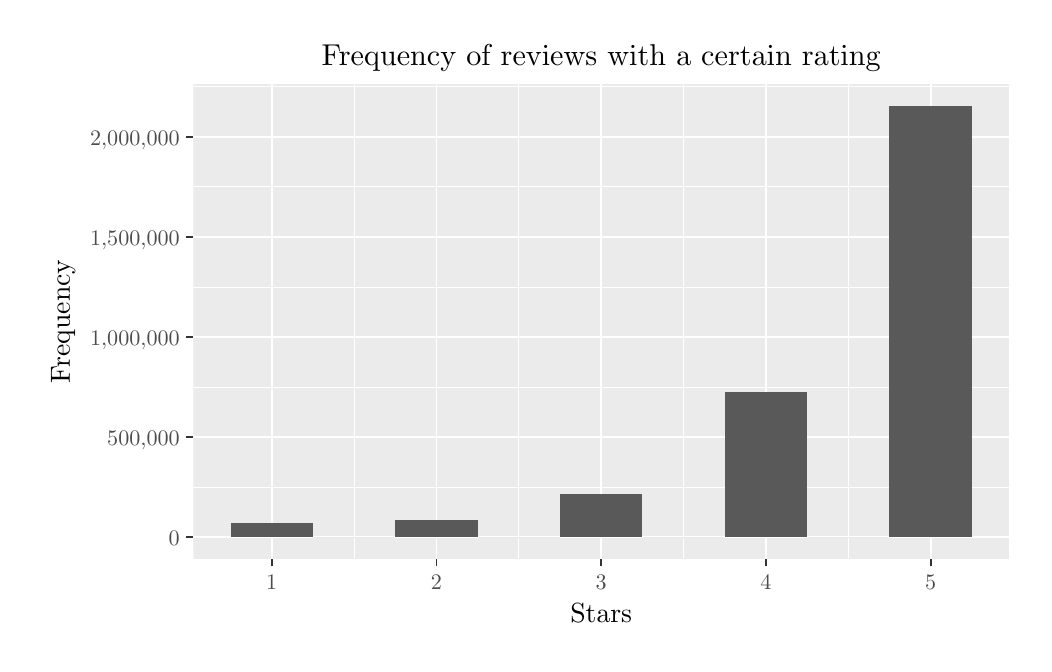
\begin{tikzpicture}[x=1pt,y=1pt]
\definecolor{fillColor}{RGB}{255,255,255}
\path[use as bounding box,fill=fillColor,fill opacity=0.00] (0,0) rectangle (360.07,222.54);
\begin{scope}
\path[clip] (  0.00,  0.00) rectangle (360.07,222.54);
\definecolor{drawColor}{RGB}{255,255,255}
\definecolor{fillColor}{RGB}{255,255,255}

\path[draw=drawColor,line width= 0.6pt,line join=round,line cap=round,fill=fillColor] (  0.00,  0.00) rectangle (360.07,222.54);
\end{scope}
\begin{scope}
\path[clip] ( 59.92, 30.62) rectangle (354.57,202.21);
\definecolor{fillColor}{gray}{0.92}

\path[fill=fillColor] ( 59.92, 30.62) rectangle (354.57,202.21);
\definecolor{drawColor}{RGB}{255,255,255}

\path[draw=drawColor,line width= 0.3pt,line join=round] ( 59.92, 56.51) --
	(354.57, 56.51);

\path[draw=drawColor,line width= 0.3pt,line join=round] ( 59.92, 92.67) --
	(354.57, 92.67);

\path[draw=drawColor,line width= 0.3pt,line join=round] ( 59.92,128.84) --
	(354.57,128.84);

\path[draw=drawColor,line width= 0.3pt,line join=round] ( 59.92,165.01) --
	(354.57,165.01);

\path[draw=drawColor,line width= 0.3pt,line join=round] ( 59.92,201.17) --
	(354.57,201.17);

\path[draw=drawColor,line width= 0.3pt,line join=round] (117.96, 30.62) --
	(117.96,202.21);

\path[draw=drawColor,line width= 0.3pt,line join=round] (177.48, 30.62) --
	(177.48,202.21);

\path[draw=drawColor,line width= 0.3pt,line join=round] (237.01, 30.62) --
	(237.01,202.21);

\path[draw=drawColor,line width= 0.3pt,line join=round] (296.53, 30.62) --
	(296.53,202.21);

\path[draw=drawColor,line width= 0.6pt,line join=round] ( 59.92, 38.42) --
	(354.57, 38.42);

\path[draw=drawColor,line width= 0.6pt,line join=round] ( 59.92, 74.59) --
	(354.57, 74.59);

\path[draw=drawColor,line width= 0.6pt,line join=round] ( 59.92,110.76) --
	(354.57,110.76);

\path[draw=drawColor,line width= 0.6pt,line join=round] ( 59.92,146.92) --
	(354.57,146.92);

\path[draw=drawColor,line width= 0.6pt,line join=round] ( 59.92,183.09) --
	(354.57,183.09);

\path[draw=drawColor,line width= 0.6pt,line join=round] ( 88.19, 30.62) --
	( 88.19,202.21);

\path[draw=drawColor,line width= 0.6pt,line join=round] (147.72, 30.62) --
	(147.72,202.21);

\path[draw=drawColor,line width= 0.6pt,line join=round] (207.25, 30.62) --
	(207.25,202.21);

\path[draw=drawColor,line width= 0.6pt,line join=round] (266.77, 30.62) --
	(266.77,202.21);

\path[draw=drawColor,line width= 0.6pt,line join=round] (326.30, 30.62) --
	(326.30,202.21);
\definecolor{fillColor}{gray}{0.35}

\path[fill=fillColor] ( 73.31, 38.42) rectangle (103.08, 43.59);

\path[fill=fillColor] (103.08, 38.42) rectangle (132.84, 38.42);

\path[fill=fillColor] (132.84, 38.42) rectangle (162.60, 44.71);

\path[fill=fillColor] (162.60, 38.42) rectangle (192.36, 38.42);

\path[fill=fillColor] (192.36, 38.42) rectangle (222.13, 53.87);

\path[fill=fillColor] (222.13, 38.42) rectangle (251.89, 38.42);

\path[fill=fillColor] (251.89, 38.42) rectangle (281.65, 90.85);

\path[fill=fillColor] (281.65, 38.42) rectangle (311.41, 38.42);

\path[fill=fillColor] (311.41, 38.42) rectangle (341.18,194.41);
\end{scope}
\begin{scope}
\path[clip] (  0.00,  0.00) rectangle (360.07,222.54);
\definecolor{drawColor}{gray}{0.30}

\node[text=drawColor,anchor=base east,inner sep=0pt, outer sep=0pt, scale=  0.80] at ( 54.97, 35.41) {0};

\node[text=drawColor,anchor=base east,inner sep=0pt, outer sep=0pt, scale=  0.80] at ( 54.97, 71.57) {500,000};

\node[text=drawColor,anchor=base east,inner sep=0pt, outer sep=0pt, scale=  0.80] at ( 54.97,107.74) {1,000,000};

\node[text=drawColor,anchor=base east,inner sep=0pt, outer sep=0pt, scale=  0.80] at ( 54.97,143.91) {1,500,000};

\node[text=drawColor,anchor=base east,inner sep=0pt, outer sep=0pt, scale=  0.80] at ( 54.97,180.07) {2,000,000};
\end{scope}
\begin{scope}
\path[clip] (  0.00,  0.00) rectangle (360.07,222.54);
\definecolor{drawColor}{gray}{0.20}

\path[draw=drawColor,line width= 0.6pt,line join=round] ( 57.17, 38.42) --
	( 59.92, 38.42);

\path[draw=drawColor,line width= 0.6pt,line join=round] ( 57.17, 74.59) --
	( 59.92, 74.59);

\path[draw=drawColor,line width= 0.6pt,line join=round] ( 57.17,110.76) --
	( 59.92,110.76);

\path[draw=drawColor,line width= 0.6pt,line join=round] ( 57.17,146.92) --
	( 59.92,146.92);

\path[draw=drawColor,line width= 0.6pt,line join=round] ( 57.17,183.09) --
	( 59.92,183.09);
\end{scope}
\begin{scope}
\path[clip] (  0.00,  0.00) rectangle (360.07,222.54);
\definecolor{drawColor}{gray}{0.20}

\path[draw=drawColor,line width= 0.6pt,line join=round] ( 88.19, 27.87) --
	( 88.19, 30.62);

\path[draw=drawColor,line width= 0.6pt,line join=round] (147.72, 27.87) --
	(147.72, 30.62);

\path[draw=drawColor,line width= 0.6pt,line join=round] (207.25, 27.87) --
	(207.25, 30.62);

\path[draw=drawColor,line width= 0.6pt,line join=round] (266.77, 27.87) --
	(266.77, 30.62);

\path[draw=drawColor,line width= 0.6pt,line join=round] (326.30, 27.87) --
	(326.30, 30.62);
\end{scope}
\begin{scope}
\path[clip] (  0.00,  0.00) rectangle (360.07,222.54);
\definecolor{drawColor}{gray}{0.30}

\node[text=drawColor,anchor=base,inner sep=0pt, outer sep=0pt, scale=  0.80] at ( 88.19, 19.64) {1};

\node[text=drawColor,anchor=base,inner sep=0pt, outer sep=0pt, scale=  0.80] at (147.72, 19.64) {2};

\node[text=drawColor,anchor=base,inner sep=0pt, outer sep=0pt, scale=  0.80] at (207.25, 19.64) {3};

\node[text=drawColor,anchor=base,inner sep=0pt, outer sep=0pt, scale=  0.80] at (266.77, 19.64) {4};

\node[text=drawColor,anchor=base,inner sep=0pt, outer sep=0pt, scale=  0.80] at (326.30, 19.64) {5};
\end{scope}
\begin{scope}
\path[clip] (  0.00,  0.00) rectangle (360.07,222.54);
\definecolor{drawColor}{RGB}{0,0,0}

\node[text=drawColor,anchor=base,inner sep=0pt, outer sep=0pt, scale=  1.00] at (207.25,  7.70) {Stars};
\end{scope}
\begin{scope}
\path[clip] (  0.00,  0.00) rectangle (360.07,222.54);
\definecolor{drawColor}{RGB}{0,0,0}

\node[text=drawColor,rotate= 90.00,anchor=base,inner sep=0pt, outer sep=0pt, scale=  1.00] at ( 15.24,116.42) {Frequency};
\end{scope}
\begin{scope}
\path[clip] (  0.00,  0.00) rectangle (360.07,222.54);
\definecolor{drawColor}{RGB}{0,0,0}

\node[text=drawColor,anchor=base,inner sep=0pt, outer sep=0pt, scale=  1.09] at (207.25,208.81) {Frequency of reviews with a certain rating};
\end{scope}
\end{tikzpicture}

	\caption{From the plot it can be seen that the vast majority of reviews give the highest rating to the recipe, which might suggest that users might be more likely to review a recipe if they are positive about it.}
	\label{fig:user_ratings}
\end{figure}

Meals with no ratings are left out of the rating matrix so that no columns have only zeros.
\cref{tab:dataset_summary}, that was previously referred to, also shows some statistics on the rating data.
About two thirds of the recipes have at least one rating.
Another observation is that the density of the rating matrix several orders of magnitudes lower, which is caused by the fact that there are many more users than ingredients and most users rate only one recipe.
This is also shown in \cref{fig:user_little_ratings}.
The majority of users only reviewed a single recipe and \SI{90}{\percent} of the users has reviewed $\leq 7$ recipes.
Knowing that many users submitted very few ratings might make it hard to make predictions about the ratings for recipes the user did not rate.
On the other hand, Allrecipes has a few very active users with the top reviewer being a user that submitted $\num{5250}$ ratings.
\cref{fig:user_many_ratings} zooms in on this end of tail and shows that is very uncommon.
In fact, only $113$ users submitted more than $\num{1000}$ reviews.

\begin{figure}[htbp]
	\centering
	% Created by tikzDevice version 0.10.1 on 2016-07-26 20:48:00
% !TEX encoding = UTF-8 Unicode
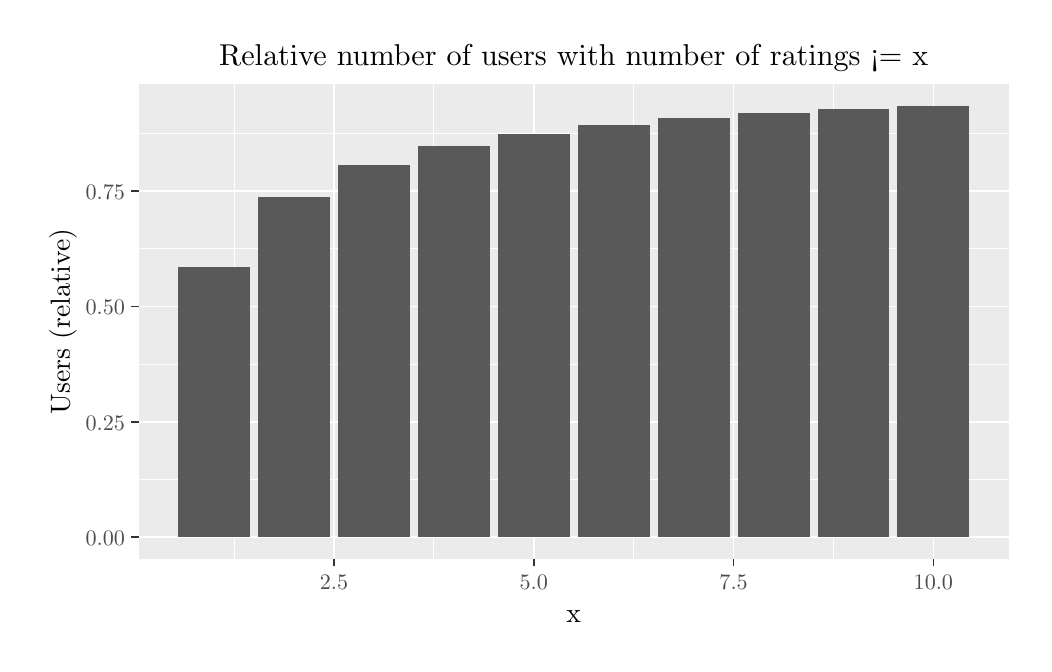
\begin{tikzpicture}[x=1pt,y=1pt]
\definecolor{fillColor}{RGB}{255,255,255}
\path[use as bounding box,fill=fillColor,fill opacity=0.00] (0,0) rectangle (360.07,222.54);
\begin{scope}
\path[clip] (  0.00,  0.00) rectangle (360.07,222.54);
\definecolor{drawColor}{RGB}{255,255,255}
\definecolor{fillColor}{RGB}{255,255,255}

\path[draw=drawColor,line width= 0.6pt,line join=round,line cap=round,fill=fillColor] (  0.00,  0.00) rectangle (360.07,222.54);
\end{scope}
\begin{scope}
\path[clip] ( 40.08, 30.62) rectangle (354.57,202.21);
\definecolor{fillColor}{gray}{0.92}

\path[fill=fillColor] ( 40.08, 30.62) rectangle (354.57,202.21);
\definecolor{drawColor}{RGB}{255,255,255}

\path[draw=drawColor,line width= 0.3pt,line join=round] ( 40.08, 59.27) --
	(354.57, 59.27);

\path[draw=drawColor,line width= 0.3pt,line join=round] ( 40.08,100.95) --
	(354.57,100.95);

\path[draw=drawColor,line width= 0.3pt,line join=round] ( 40.08,142.64) --
	(354.57,142.64);

\path[draw=drawColor,line width= 0.3pt,line join=round] ( 40.08,184.33) --
	(354.57,184.33);

\path[draw=drawColor,line width= 0.3pt,line join=round] ( 74.59, 30.62) --
	( 74.59,202.21);

\path[draw=drawColor,line width= 0.3pt,line join=round] (146.79, 30.62) --
	(146.79,202.21);

\path[draw=drawColor,line width= 0.3pt,line join=round] (218.98, 30.62) --
	(218.98,202.21);

\path[draw=drawColor,line width= 0.3pt,line join=round] (291.18, 30.62) --
	(291.18,202.21);

\path[draw=drawColor,line width= 0.6pt,line join=round] ( 40.08, 38.42) --
	(354.57, 38.42);

\path[draw=drawColor,line width= 0.6pt,line join=round] ( 40.08, 80.11) --
	(354.57, 80.11);

\path[draw=drawColor,line width= 0.6pt,line join=round] ( 40.08,121.80) --
	(354.57,121.80);

\path[draw=drawColor,line width= 0.6pt,line join=round] ( 40.08,163.48) --
	(354.57,163.48);

\path[draw=drawColor,line width= 0.6pt,line join=round] (110.69, 30.62) --
	(110.69,202.21);

\path[draw=drawColor,line width= 0.6pt,line join=round] (182.88, 30.62) --
	(182.88,202.21);

\path[draw=drawColor,line width= 0.6pt,line join=round] (255.08, 30.62) --
	(255.08,202.21);

\path[draw=drawColor,line width= 0.6pt,line join=round] (327.28, 30.62) --
	(327.28,202.21);
\definecolor{fillColor}{gray}{0.35}

\path[fill=fillColor] ( 54.37, 38.42) rectangle ( 80.36,136.20);

\path[fill=fillColor] ( 83.25, 38.42) rectangle (109.24,161.22);

\path[fill=fillColor] (112.13, 38.42) rectangle (138.12,172.82);

\path[fill=fillColor] (141.01, 38.42) rectangle (167.00,179.68);

\path[fill=fillColor] (169.89, 38.42) rectangle (195.88,184.16);

\path[fill=fillColor] (198.77, 38.42) rectangle (224.76,187.38);

\path[fill=fillColor] (227.65, 38.42) rectangle (253.64,189.82);

\path[fill=fillColor] (256.53, 38.42) rectangle (282.52,191.71);

\path[fill=fillColor] (285.41, 38.42) rectangle (311.40,193.18);

\path[fill=fillColor] (314.28, 38.42) rectangle (340.28,194.41);
\end{scope}
\begin{scope}
\path[clip] (  0.00,  0.00) rectangle (360.07,222.54);
\definecolor{drawColor}{gray}{0.30}

\node[text=drawColor,anchor=base east,inner sep=0pt, outer sep=0pt, scale=  0.80] at ( 35.13, 35.41) {0.00};

\node[text=drawColor,anchor=base east,inner sep=0pt, outer sep=0pt, scale=  0.80] at ( 35.13, 77.09) {0.25};

\node[text=drawColor,anchor=base east,inner sep=0pt, outer sep=0pt, scale=  0.80] at ( 35.13,118.78) {0.50};

\node[text=drawColor,anchor=base east,inner sep=0pt, outer sep=0pt, scale=  0.80] at ( 35.13,160.47) {0.75};
\end{scope}
\begin{scope}
\path[clip] (  0.00,  0.00) rectangle (360.07,222.54);
\definecolor{drawColor}{gray}{0.20}

\path[draw=drawColor,line width= 0.6pt,line join=round] ( 37.33, 38.42) --
	( 40.08, 38.42);

\path[draw=drawColor,line width= 0.6pt,line join=round] ( 37.33, 80.11) --
	( 40.08, 80.11);

\path[draw=drawColor,line width= 0.6pt,line join=round] ( 37.33,121.80) --
	( 40.08,121.80);

\path[draw=drawColor,line width= 0.6pt,line join=round] ( 37.33,163.48) --
	( 40.08,163.48);
\end{scope}
\begin{scope}
\path[clip] (  0.00,  0.00) rectangle (360.07,222.54);
\definecolor{drawColor}{gray}{0.20}

\path[draw=drawColor,line width= 0.6pt,line join=round] (110.69, 27.87) --
	(110.69, 30.62);

\path[draw=drawColor,line width= 0.6pt,line join=round] (182.88, 27.87) --
	(182.88, 30.62);

\path[draw=drawColor,line width= 0.6pt,line join=round] (255.08, 27.87) --
	(255.08, 30.62);

\path[draw=drawColor,line width= 0.6pt,line join=round] (327.28, 27.87) --
	(327.28, 30.62);
\end{scope}
\begin{scope}
\path[clip] (  0.00,  0.00) rectangle (360.07,222.54);
\definecolor{drawColor}{gray}{0.30}

\node[text=drawColor,anchor=base,inner sep=0pt, outer sep=0pt, scale=  0.80] at (110.69, 19.64) {2.5};

\node[text=drawColor,anchor=base,inner sep=0pt, outer sep=0pt, scale=  0.80] at (182.88, 19.64) {5.0};

\node[text=drawColor,anchor=base,inner sep=0pt, outer sep=0pt, scale=  0.80] at (255.08, 19.64) {7.5};

\node[text=drawColor,anchor=base,inner sep=0pt, outer sep=0pt, scale=  0.80] at (327.28, 19.64) {10.0};
\end{scope}
\begin{scope}
\path[clip] (  0.00,  0.00) rectangle (360.07,222.54);
\definecolor{drawColor}{RGB}{0,0,0}

\node[text=drawColor,anchor=base,inner sep=0pt, outer sep=0pt, scale=  1.00] at (197.32,  7.70) {x};
\end{scope}
\begin{scope}
\path[clip] (  0.00,  0.00) rectangle (360.07,222.54);
\definecolor{drawColor}{RGB}{0,0,0}

\node[text=drawColor,rotate= 90.00,anchor=base,inner sep=0pt, outer sep=0pt, scale=  1.00] at ( 15.24,116.42) {Users (relative)};
\end{scope}
\begin{scope}
\path[clip] (  0.00,  0.00) rectangle (360.07,222.54);
\definecolor{drawColor}{RGB}{0,0,0}

\node[text=drawColor,anchor=base,inner sep=0pt, outer sep=0pt, scale=  1.09] at (197.32,208.81) {Relative number of users with number of ratings <= x};
\end{scope}
\end{tikzpicture}

	\caption{The number of people with only a few ratings is large, though this is rather common. Approximately \SI{58}{\percent} of the users only rated one recipe, while \SI{94}{\percent} of users rated $\leq 10$ recipes.}
	\label{fig:user_little_ratings}
\end{figure}

\begin{figure}[htbp]
	\centering
	% Created by tikzDevice version 0.10.1 on 2016-07-26 22:19:47
% !TEX encoding = UTF-8 Unicode
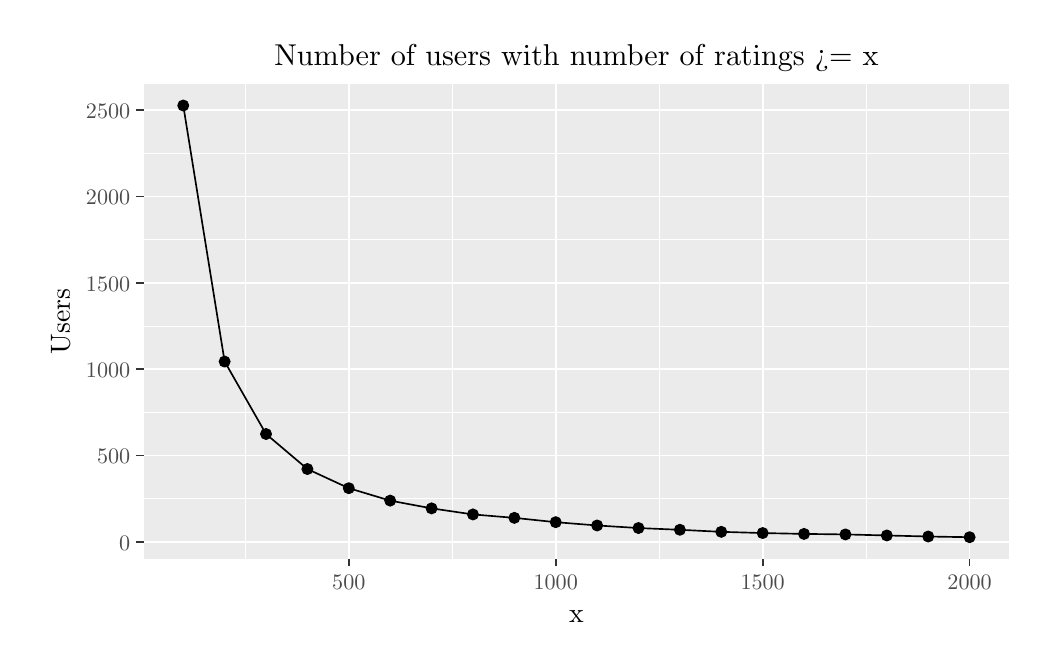
\begin{tikzpicture}[x=1pt,y=1pt]
\definecolor{fillColor}{RGB}{255,255,255}
\path[use as bounding box,fill=fillColor,fill opacity=0.00] (0,0) rectangle (360.07,222.54);
\begin{scope}
\path[clip] (  0.00,  0.00) rectangle (360.07,222.54);
\definecolor{drawColor}{RGB}{255,255,255}
\definecolor{fillColor}{RGB}{255,255,255}

\path[draw=drawColor,line width= 0.6pt,line join=round,line cap=round,fill=fillColor] (  0.00,  0.00) rectangle (360.07,222.54);
\end{scope}
\begin{scope}
\path[clip] ( 42.01, 30.62) rectangle (354.57,202.21);
\definecolor{fillColor}{gray}{0.92}

\path[fill=fillColor] ( 42.01, 30.62) rectangle (354.57,202.21);
\definecolor{drawColor}{RGB}{255,255,255}

\path[draw=drawColor,line width= 0.3pt,line join=round] ( 42.01, 52.39) --
	(354.57, 52.39);

\path[draw=drawColor,line width= 0.3pt,line join=round] ( 42.01, 83.56) --
	(354.57, 83.56);

\path[draw=drawColor,line width= 0.3pt,line join=round] ( 42.01,114.74) --
	(354.57,114.74);

\path[draw=drawColor,line width= 0.3pt,line join=round] ( 42.01,145.91) --
	(354.57,145.91);

\path[draw=drawColor,line width= 0.3pt,line join=round] ( 42.01,177.08) --
	(354.57,177.08);

\path[draw=drawColor,line width= 0.3pt,line join=round] ( 78.65, 30.62) --
	( 78.65,202.21);

\path[draw=drawColor,line width= 0.3pt,line join=round] (153.43, 30.62) --
	(153.43,202.21);

\path[draw=drawColor,line width= 0.3pt,line join=round] (228.20, 30.62) --
	(228.20,202.21);

\path[draw=drawColor,line width= 0.3pt,line join=round] (302.98, 30.62) --
	(302.98,202.21);

\path[draw=drawColor,line width= 0.6pt,line join=round] ( 42.01, 36.80) --
	(354.57, 36.80);

\path[draw=drawColor,line width= 0.6pt,line join=round] ( 42.01, 67.98) --
	(354.57, 67.98);

\path[draw=drawColor,line width= 0.6pt,line join=round] ( 42.01, 99.15) --
	(354.57, 99.15);

\path[draw=drawColor,line width= 0.6pt,line join=round] ( 42.01,130.32) --
	(354.57,130.32);

\path[draw=drawColor,line width= 0.6pt,line join=round] ( 42.01,161.49) --
	(354.57,161.49);

\path[draw=drawColor,line width= 0.6pt,line join=round] ( 42.01,192.67) --
	(354.57,192.67);

\path[draw=drawColor,line width= 0.6pt,line join=round] (116.04, 30.62) --
	(116.04,202.21);

\path[draw=drawColor,line width= 0.6pt,line join=round] (190.81, 30.62) --
	(190.81,202.21);

\path[draw=drawColor,line width= 0.6pt,line join=round] (265.59, 30.62) --
	(265.59,202.21);

\path[draw=drawColor,line width= 0.6pt,line join=round] (340.36, 30.62) --
	(340.36,202.21);
\definecolor{drawColor}{RGB}{0,0,0}

\path[draw=drawColor,line width= 0.6pt,line join=round] ( 56.22,194.41) --
	( 71.17,101.89) --
	( 86.13, 75.71) --
	(101.08, 63.05) --
	(116.04, 56.13) --
	(130.99, 51.64) --
	(145.95, 48.84) --
	(160.90, 46.65) --
	(175.86, 45.41) --
	(190.81, 43.85) --
	(205.77, 42.66) --
	(220.72, 41.73) --
	(235.68, 41.10) --
	(250.63, 40.36) --
	(265.59, 39.92) --
	(280.54, 39.61) --
	(295.50, 39.42) --
	(310.45, 39.05) --
	(325.41, 38.67) --
	(340.36, 38.42);
\definecolor{fillColor}{RGB}{0,0,0}

\path[draw=drawColor,line width= 0.4pt,line join=round,line cap=round,fill=fillColor] ( 56.22,194.41) circle (  1.96);

\path[draw=drawColor,line width= 0.4pt,line join=round,line cap=round,fill=fillColor] ( 71.17,101.89) circle (  1.96);

\path[draw=drawColor,line width= 0.4pt,line join=round,line cap=round,fill=fillColor] ( 86.13, 75.71) circle (  1.96);

\path[draw=drawColor,line width= 0.4pt,line join=round,line cap=round,fill=fillColor] (101.08, 63.05) circle (  1.96);

\path[draw=drawColor,line width= 0.4pt,line join=round,line cap=round,fill=fillColor] (116.04, 56.13) circle (  1.96);

\path[draw=drawColor,line width= 0.4pt,line join=round,line cap=round,fill=fillColor] (130.99, 51.64) circle (  1.96);

\path[draw=drawColor,line width= 0.4pt,line join=round,line cap=round,fill=fillColor] (145.95, 48.84) circle (  1.96);

\path[draw=drawColor,line width= 0.4pt,line join=round,line cap=round,fill=fillColor] (160.90, 46.65) circle (  1.96);

\path[draw=drawColor,line width= 0.4pt,line join=round,line cap=round,fill=fillColor] (175.86, 45.41) circle (  1.96);

\path[draw=drawColor,line width= 0.4pt,line join=round,line cap=round,fill=fillColor] (190.81, 43.85) circle (  1.96);

\path[draw=drawColor,line width= 0.4pt,line join=round,line cap=round,fill=fillColor] (205.77, 42.66) circle (  1.96);

\path[draw=drawColor,line width= 0.4pt,line join=round,line cap=round,fill=fillColor] (220.72, 41.73) circle (  1.96);

\path[draw=drawColor,line width= 0.4pt,line join=round,line cap=round,fill=fillColor] (235.68, 41.10) circle (  1.96);

\path[draw=drawColor,line width= 0.4pt,line join=round,line cap=round,fill=fillColor] (250.63, 40.36) circle (  1.96);

\path[draw=drawColor,line width= 0.4pt,line join=round,line cap=round,fill=fillColor] (265.59, 39.92) circle (  1.96);

\path[draw=drawColor,line width= 0.4pt,line join=round,line cap=round,fill=fillColor] (280.54, 39.61) circle (  1.96);

\path[draw=drawColor,line width= 0.4pt,line join=round,line cap=round,fill=fillColor] (295.50, 39.42) circle (  1.96);

\path[draw=drawColor,line width= 0.4pt,line join=round,line cap=round,fill=fillColor] (310.45, 39.05) circle (  1.96);

\path[draw=drawColor,line width= 0.4pt,line join=round,line cap=round,fill=fillColor] (325.41, 38.67) circle (  1.96);

\path[draw=drawColor,line width= 0.4pt,line join=round,line cap=round,fill=fillColor] (340.36, 38.42) circle (  1.96);
\end{scope}
\begin{scope}
\path[clip] (  0.00,  0.00) rectangle (360.07,222.54);
\definecolor{drawColor}{gray}{0.30}

\node[text=drawColor,anchor=base east,inner sep=0pt, outer sep=0pt, scale=  0.80] at ( 37.06, 33.79) {0};

\node[text=drawColor,anchor=base east,inner sep=0pt, outer sep=0pt, scale=  0.80] at ( 37.06, 64.96) {500};

\node[text=drawColor,anchor=base east,inner sep=0pt, outer sep=0pt, scale=  0.80] at ( 37.06, 96.13) {1000};

\node[text=drawColor,anchor=base east,inner sep=0pt, outer sep=0pt, scale=  0.80] at ( 37.06,127.31) {1500};

\node[text=drawColor,anchor=base east,inner sep=0pt, outer sep=0pt, scale=  0.80] at ( 37.06,158.48) {2000};

\node[text=drawColor,anchor=base east,inner sep=0pt, outer sep=0pt, scale=  0.80] at ( 37.06,189.65) {2500};
\end{scope}
\begin{scope}
\path[clip] (  0.00,  0.00) rectangle (360.07,222.54);
\definecolor{drawColor}{gray}{0.20}

\path[draw=drawColor,line width= 0.6pt,line join=round] ( 39.26, 36.80) --
	( 42.01, 36.80);

\path[draw=drawColor,line width= 0.6pt,line join=round] ( 39.26, 67.98) --
	( 42.01, 67.98);

\path[draw=drawColor,line width= 0.6pt,line join=round] ( 39.26, 99.15) --
	( 42.01, 99.15);

\path[draw=drawColor,line width= 0.6pt,line join=round] ( 39.26,130.32) --
	( 42.01,130.32);

\path[draw=drawColor,line width= 0.6pt,line join=round] ( 39.26,161.49) --
	( 42.01,161.49);

\path[draw=drawColor,line width= 0.6pt,line join=round] ( 39.26,192.67) --
	( 42.01,192.67);
\end{scope}
\begin{scope}
\path[clip] (  0.00,  0.00) rectangle (360.07,222.54);
\definecolor{drawColor}{gray}{0.20}

\path[draw=drawColor,line width= 0.6pt,line join=round] (116.04, 27.87) --
	(116.04, 30.62);

\path[draw=drawColor,line width= 0.6pt,line join=round] (190.81, 27.87) --
	(190.81, 30.62);

\path[draw=drawColor,line width= 0.6pt,line join=round] (265.59, 27.87) --
	(265.59, 30.62);

\path[draw=drawColor,line width= 0.6pt,line join=round] (340.36, 27.87) --
	(340.36, 30.62);
\end{scope}
\begin{scope}
\path[clip] (  0.00,  0.00) rectangle (360.07,222.54);
\definecolor{drawColor}{gray}{0.30}

\node[text=drawColor,anchor=base,inner sep=0pt, outer sep=0pt, scale=  0.80] at (116.04, 19.64) {500};

\node[text=drawColor,anchor=base,inner sep=0pt, outer sep=0pt, scale=  0.80] at (190.81, 19.64) {1000};

\node[text=drawColor,anchor=base,inner sep=0pt, outer sep=0pt, scale=  0.80] at (265.59, 19.64) {1500};

\node[text=drawColor,anchor=base,inner sep=0pt, outer sep=0pt, scale=  0.80] at (340.36, 19.64) {2000};
\end{scope}
\begin{scope}
\path[clip] (  0.00,  0.00) rectangle (360.07,222.54);
\definecolor{drawColor}{RGB}{0,0,0}

\node[text=drawColor,anchor=base,inner sep=0pt, outer sep=0pt, scale=  1.00] at (198.29,  7.70) {x};
\end{scope}
\begin{scope}
\path[clip] (  0.00,  0.00) rectangle (360.07,222.54);
\definecolor{drawColor}{RGB}{0,0,0}

\node[text=drawColor,rotate= 90.00,anchor=base,inner sep=0pt, outer sep=0pt, scale=  1.00] at ( 15.24,116.42) {Users};
\end{scope}
\begin{scope}
\path[clip] (  0.00,  0.00) rectangle (360.07,222.54);
\definecolor{drawColor}{RGB}{0,0,0}

\node[text=drawColor,anchor=base,inner sep=0pt, outer sep=0pt, scale=  1.09] at (198.29,208.81) {Number of users with number of ratings >= x};
\end{scope}
\end{tikzpicture}

	\caption{There are a few users that submitted many ratings, but only $113$ users rated more than $1000$ recipes. One user even submitted $\num{5250}$ ratings.}
	\label{fig:user_many_ratings}
\end{figure}

\cref{fig:user_ratings} shows the number of reviews per score.
It seems that Allrecipes has a strong bias towards positive reviews, which might indicate that people tend to rate recipes that they appreciated.
Another explanation could be that people probably submit their favorite recipes, that are more likely to receive positive feedback.
Whatever the reason, the plot show that a difference between a $4$ and $5$ star rating is big.
One way to deal with this is to convert the rating matrix into a binary matrix $\hat{R}$:

\begin{equation*}
	\tag{Binary Rating matrix}
	\hat{R}_{ij}=
	\begin{cases}
	    1,& \text{if } R_{ij}>t \\
	    0,& \text{otherwise}
	\end{cases}
\end{equation*}

\begin{figure}[htbp]
	\centering
	% Created by tikzDevice version 0.10.1 on 2016-08-02 18:36:23
% !TEX encoding = UTF-8 Unicode
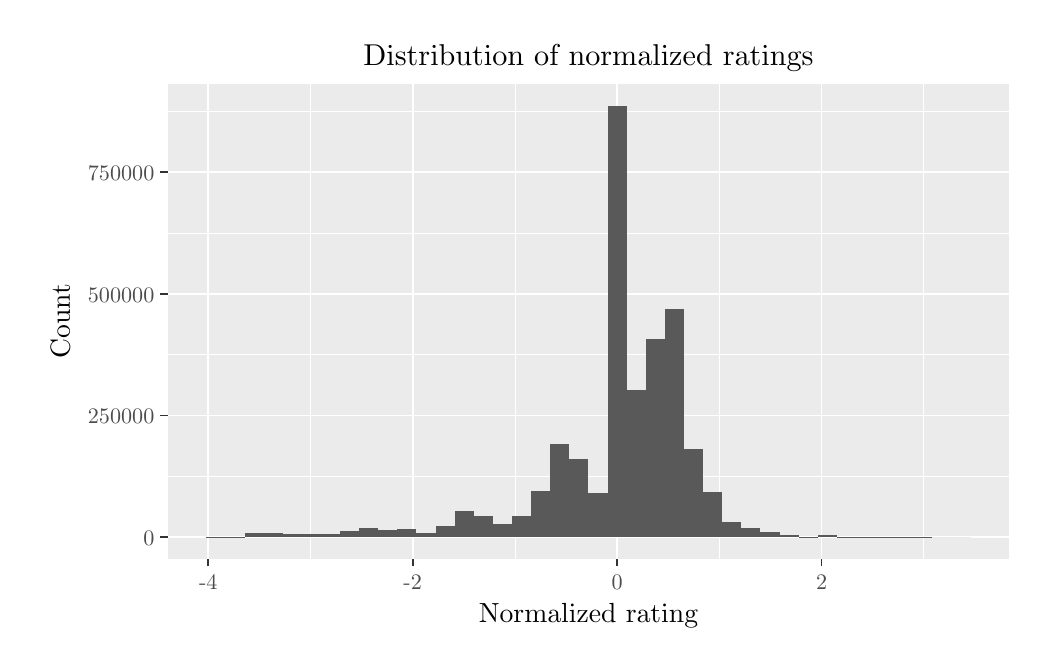
\begin{tikzpicture}[x=1pt,y=1pt]
\definecolor{fillColor}{RGB}{255,255,255}
\path[use as bounding box,fill=fillColor,fill opacity=0.00] (0,0) rectangle (360.07,222.54);
\begin{scope}
\path[clip] (  0.00,  0.00) rectangle (360.07,222.54);
\definecolor{drawColor}{RGB}{255,255,255}
\definecolor{fillColor}{RGB}{255,255,255}

\path[draw=drawColor,line width= 0.6pt,line join=round,line cap=round,fill=fillColor] (  0.00,  0.00) rectangle (360.07,222.54);
\end{scope}
\begin{scope}
\path[clip] ( 50.72, 30.62) rectangle (354.57,202.21);
\definecolor{fillColor}{gray}{0.92}

\path[fill=fillColor] ( 50.72, 30.62) rectangle (354.57,202.21);
\definecolor{drawColor}{RGB}{255,255,255}

\path[draw=drawColor,line width= 0.3pt,line join=round] ( 50.72, 60.40) --
	(354.57, 60.40);

\path[draw=drawColor,line width= 0.3pt,line join=round] ( 50.72,104.37) --
	(354.57,104.37);

\path[draw=drawColor,line width= 0.3pt,line join=round] ( 50.72,148.33) --
	(354.57,148.33);

\path[draw=drawColor,line width= 0.3pt,line join=round] ( 50.72,192.29) --
	(354.57,192.29);

\path[draw=drawColor,line width= 0.3pt,line join=round] (102.19, 30.62) --
	(102.19,202.21);

\path[draw=drawColor,line width= 0.3pt,line join=round] (176.07, 30.62) --
	(176.07,202.21);

\path[draw=drawColor,line width= 0.3pt,line join=round] (249.94, 30.62) --
	(249.94,202.21);

\path[draw=drawColor,line width= 0.3pt,line join=round] (323.82, 30.62) --
	(323.82,202.21);

\path[draw=drawColor,line width= 0.6pt,line join=round] ( 50.72, 38.42) --
	(354.57, 38.42);

\path[draw=drawColor,line width= 0.6pt,line join=round] ( 50.72, 82.39) --
	(354.57, 82.39);

\path[draw=drawColor,line width= 0.6pt,line join=round] ( 50.72,126.35) --
	(354.57,126.35);

\path[draw=drawColor,line width= 0.6pt,line join=round] ( 50.72,170.31) --
	(354.57,170.31);

\path[draw=drawColor,line width= 0.6pt,line join=round] ( 65.26, 30.62) --
	( 65.26,202.21);

\path[draw=drawColor,line width= 0.6pt,line join=round] (139.13, 30.62) --
	(139.13,202.21);

\path[draw=drawColor,line width= 0.6pt,line join=round] (213.01, 30.62) --
	(213.01,202.21);

\path[draw=drawColor,line width= 0.6pt,line join=round] (286.88, 30.62) --
	(286.88,202.21);
\definecolor{fillColor}{gray}{0.35}

\path[fill=fillColor] ( 64.53, 38.42) rectangle ( 71.44, 38.44);

\path[fill=fillColor] ( 71.44, 38.42) rectangle ( 78.35, 38.67);

\path[fill=fillColor] ( 78.35, 38.42) rectangle ( 85.25, 40.09);

\path[fill=fillColor] ( 85.25, 38.42) rectangle ( 92.16, 40.07);

\path[fill=fillColor] ( 92.16, 38.42) rectangle ( 99.06, 39.54);

\path[fill=fillColor] ( 99.06, 38.42) rectangle (105.97, 39.45);

\path[fill=fillColor] (105.97, 38.42) rectangle (112.87, 39.41);

\path[fill=fillColor] (112.87, 38.42) rectangle (119.78, 40.49);

\path[fill=fillColor] (119.78, 38.42) rectangle (126.68, 41.79);

\path[fill=fillColor] (126.68, 38.42) rectangle (133.59, 41.05);

\path[fill=fillColor] (133.59, 38.42) rectangle (140.50, 41.29);

\path[fill=fillColor] (140.50, 38.42) rectangle (147.40, 40.11);

\path[fill=fillColor] (147.40, 38.42) rectangle (154.31, 42.40);

\path[fill=fillColor] (154.31, 38.42) rectangle (161.21, 48.01);

\path[fill=fillColor] (161.21, 38.42) rectangle (168.12, 46.17);

\path[fill=fillColor] (168.12, 38.42) rectangle (175.02, 43.34);

\path[fill=fillColor] (175.02, 38.42) rectangle (181.93, 46.09);

\path[fill=fillColor] (181.93, 38.42) rectangle (188.84, 55.10);

\path[fill=fillColor] (188.84, 38.42) rectangle (195.74, 72.23);

\path[fill=fillColor] (195.74, 38.42) rectangle (202.65, 66.56);

\path[fill=fillColor] (202.65, 38.42) rectangle (209.55, 54.50);

\path[fill=fillColor] (209.55, 38.42) rectangle (216.46,194.41);

\path[fill=fillColor] (216.46, 38.42) rectangle (223.36, 91.46);

\path[fill=fillColor] (223.36, 38.42) rectangle (230.27,110.16);

\path[fill=fillColor] (230.27, 38.42) rectangle (237.17,121.05);

\path[fill=fillColor] (237.17, 38.42) rectangle (244.08, 70.36);

\path[fill=fillColor] (244.08, 38.42) rectangle (250.99, 54.76);

\path[fill=fillColor] (250.99, 38.42) rectangle (257.89, 43.79);

\path[fill=fillColor] (257.89, 38.42) rectangle (264.80, 41.84);

\path[fill=fillColor] (264.80, 38.42) rectangle (271.70, 40.23);

\path[fill=fillColor] (271.70, 38.42) rectangle (278.61, 39.18);

\path[fill=fillColor] (278.61, 38.42) rectangle (285.51, 38.63);

\path[fill=fillColor] (285.51, 38.42) rectangle (292.42, 39.25);

\path[fill=fillColor] (292.42, 38.42) rectangle (299.33, 38.52);

\path[fill=fillColor] (299.33, 38.42) rectangle (306.23, 38.45);

\path[fill=fillColor] (306.23, 38.42) rectangle (313.14, 38.46);

\path[fill=fillColor] (313.14, 38.42) rectangle (320.04, 38.43);

\path[fill=fillColor] (320.04, 38.42) rectangle (326.95, 38.43);

\path[fill=fillColor] (326.95, 38.42) rectangle (333.85, 38.42);

\path[fill=fillColor] (333.85, 38.42) rectangle (340.76, 38.42);
\end{scope}
\begin{scope}
\path[clip] (  0.00,  0.00) rectangle (360.07,222.54);
\definecolor{drawColor}{gray}{0.30}

\node[text=drawColor,anchor=base east,inner sep=0pt, outer sep=0pt, scale=  0.80] at ( 45.77, 35.41) {0};

\node[text=drawColor,anchor=base east,inner sep=0pt, outer sep=0pt, scale=  0.80] at ( 45.77, 79.37) {250000};

\node[text=drawColor,anchor=base east,inner sep=0pt, outer sep=0pt, scale=  0.80] at ( 45.77,123.33) {500000};

\node[text=drawColor,anchor=base east,inner sep=0pt, outer sep=0pt, scale=  0.80] at ( 45.77,167.29) {750000};
\end{scope}
\begin{scope}
\path[clip] (  0.00,  0.00) rectangle (360.07,222.54);
\definecolor{drawColor}{gray}{0.20}

\path[draw=drawColor,line width= 0.6pt,line join=round] ( 47.97, 38.42) --
	( 50.72, 38.42);

\path[draw=drawColor,line width= 0.6pt,line join=round] ( 47.97, 82.39) --
	( 50.72, 82.39);

\path[draw=drawColor,line width= 0.6pt,line join=round] ( 47.97,126.35) --
	( 50.72,126.35);

\path[draw=drawColor,line width= 0.6pt,line join=round] ( 47.97,170.31) --
	( 50.72,170.31);
\end{scope}
\begin{scope}
\path[clip] (  0.00,  0.00) rectangle (360.07,222.54);
\definecolor{drawColor}{gray}{0.20}

\path[draw=drawColor,line width= 0.6pt,line join=round] ( 65.26, 27.87) --
	( 65.26, 30.62);

\path[draw=drawColor,line width= 0.6pt,line join=round] (139.13, 27.87) --
	(139.13, 30.62);

\path[draw=drawColor,line width= 0.6pt,line join=round] (213.01, 27.87) --
	(213.01, 30.62);

\path[draw=drawColor,line width= 0.6pt,line join=round] (286.88, 27.87) --
	(286.88, 30.62);
\end{scope}
\begin{scope}
\path[clip] (  0.00,  0.00) rectangle (360.07,222.54);
\definecolor{drawColor}{gray}{0.30}

\node[text=drawColor,anchor=base,inner sep=0pt, outer sep=0pt, scale=  0.80] at ( 65.26, 19.64) {-4};

\node[text=drawColor,anchor=base,inner sep=0pt, outer sep=0pt, scale=  0.80] at (139.13, 19.64) {-2};

\node[text=drawColor,anchor=base,inner sep=0pt, outer sep=0pt, scale=  0.80] at (213.01, 19.64) {0};

\node[text=drawColor,anchor=base,inner sep=0pt, outer sep=0pt, scale=  0.80] at (286.88, 19.64) {2};
\end{scope}
\begin{scope}
\path[clip] (  0.00,  0.00) rectangle (360.07,222.54);
\definecolor{drawColor}{RGB}{0,0,0}

\node[text=drawColor,anchor=base,inner sep=0pt, outer sep=0pt, scale=  1.00] at (202.65,  7.70) {Normalized rating};
\end{scope}
\begin{scope}
\path[clip] (  0.00,  0.00) rectangle (360.07,222.54);
\definecolor{drawColor}{RGB}{0,0,0}

\node[text=drawColor,rotate= 90.00,anchor=base,inner sep=0pt, outer sep=0pt, scale=  1.00] at ( 15.24,116.42) {Count};
\end{scope}
\begin{scope}
\path[clip] (  0.00,  0.00) rectangle (360.07,222.54);
\definecolor{drawColor}{RGB}{0,0,0}

\node[text=drawColor,anchor=base,inner sep=0pt, outer sep=0pt, scale=  1.09] at (202.65,208.81) {Distribution of normalized ratings};
\end{scope}
\end{tikzpicture}

	\caption{Normalizing the user ratings using their average rating reveals that users tend to give most recipes that they review their average rating and a only small proportion a slightly less positive or negative rating (with a bias towards positive).}
	\label{fig:normalized_ratings}
\end{figure}

\noindent where $t \in S$ is a threshold on the rating value.
Another option is to normalize the rating matrix by subtracting the user bias, e.g. a user's average rating.
\cref{fig:normalized_ratings} shows the histogram of ratings after applying this transformation.
It looks like a mixture of two gaussian distributions, one for positive and one for negative feedback, with a strong peak at the user's average rating.
The deviation from the average rating is very small, with deviations $>1$ star being rare.
The clusters defined by two different distributions are interesting for to analyze in further detail.


%%%%%%%%%%%%%%%%%%%%%%%%%%%%%%%%%%%%%%%%%%%%%%%%%%%%%%%%%%%%%


\section{Data Mining}
\label{sec:data_mining}

This section describes the experiments that were performed on the datasets to obtain a better understanding of what makes a good recipe.
First, the itemsets of ingredients is mined for general patterns using association rule mining.
After that, the dataset is divided into two clusters, a positive and negative dataset, using the rating dataset.
A decision tree model is then used to learn a decision boundary between these two clusters, which is then analyzed in detail.